\chapter{Ethical development}\label{ch_EthicalDev}

\begin{chapsumm}
\cstitle{This chapter at a glance}
\begin{itemize}
\item The machine learning cycle - feedback from models to data
\item Bias measurement and interventions in the model development life cycle
\item A taxonomy of common causes of bias
\item Model governance and ethical risk management
\end{itemize}
\end{chapsumm}
%
\noindent
%
In this chapter, we transition to a more systematic approach to understanding the problems and solutions of fairness in decisions making systems. In later chapters we will look at different measures of unfairness and mitigation techniques but before we discuss and analyse these methods we review some more practical aspects of responsible model development. None of the interventions to mitigate bias that we will talk about in this book are capable of fixing a poorly formulated, discriminatory  machine learning problem so we'll start by looking at the machine learning cycle and discuss the importance of how a model is used. We'll discuss where in the machine learning model development cycle bias metrics and interventions fit and we'll classify the most common causes of bias, identifying the parts of the workflow to which they correspond. A model in itself is not the source of unfair or illegal discrimination, models are developed and deployed by people as part of a process. In order to address the problem of unfair bias we need to look at the whole system, not just the model. The methods we discuss in this book for measuring and mitigating bias won't remedy negligent deployment or management of a machine learning system. Where models can be harmful we should expect to have processes in place that aim to avoid common, foreseeable or catastrophic failures. We'll discuss how to take a proactive rather than reactive approach to managing risks associated with models.

In this chapter, we will present problems and interventions schematically. We provide a set of references for building, reviewing and monitoring machine learning solutions that aim to avoid the common pitfalls that result in biased models. We take a high enough view that the discussion remains applicable to many machine learning applications. The specifics of the framework, can be tailored for a particular application. Indeed the hope is that the resources in this chapter can be used as a starting point for data science teams that want to develop their own set of standards. Together we will progress towards thinking critically about the whole machine learning cycle, development, validation and monitoring of machine learning systems.  By the end of this chapter we will have a clearer picture of what due diligence in model development and deployment (with respect to fairness and discrimination) might look like, from a practical perspective.

%%%%%%%%%%%%%%%%%%%%%%%%%%%%%%%%%%%%%%%%%%%%%%%%%%%%%%%%%%%%%%%%%%%%%%%%%%%%
%%%%%%%%%%%%%%%%%%%%%%%%%%%%%%%%%%%%%%%%%%%%%%%%%%%%%%%%%%%%%%%%%%%%%%%%%%%%
%%%%%%%%%%%%%%%%%%%%%%%%%%%%%%%%%%%%%%%%%%%%%%%%%%%%%%%%%%%%%%%%%%%%%%%%%%%%
\section{Machine Learning Cycle}

\begin{figure}[h!]
\centering
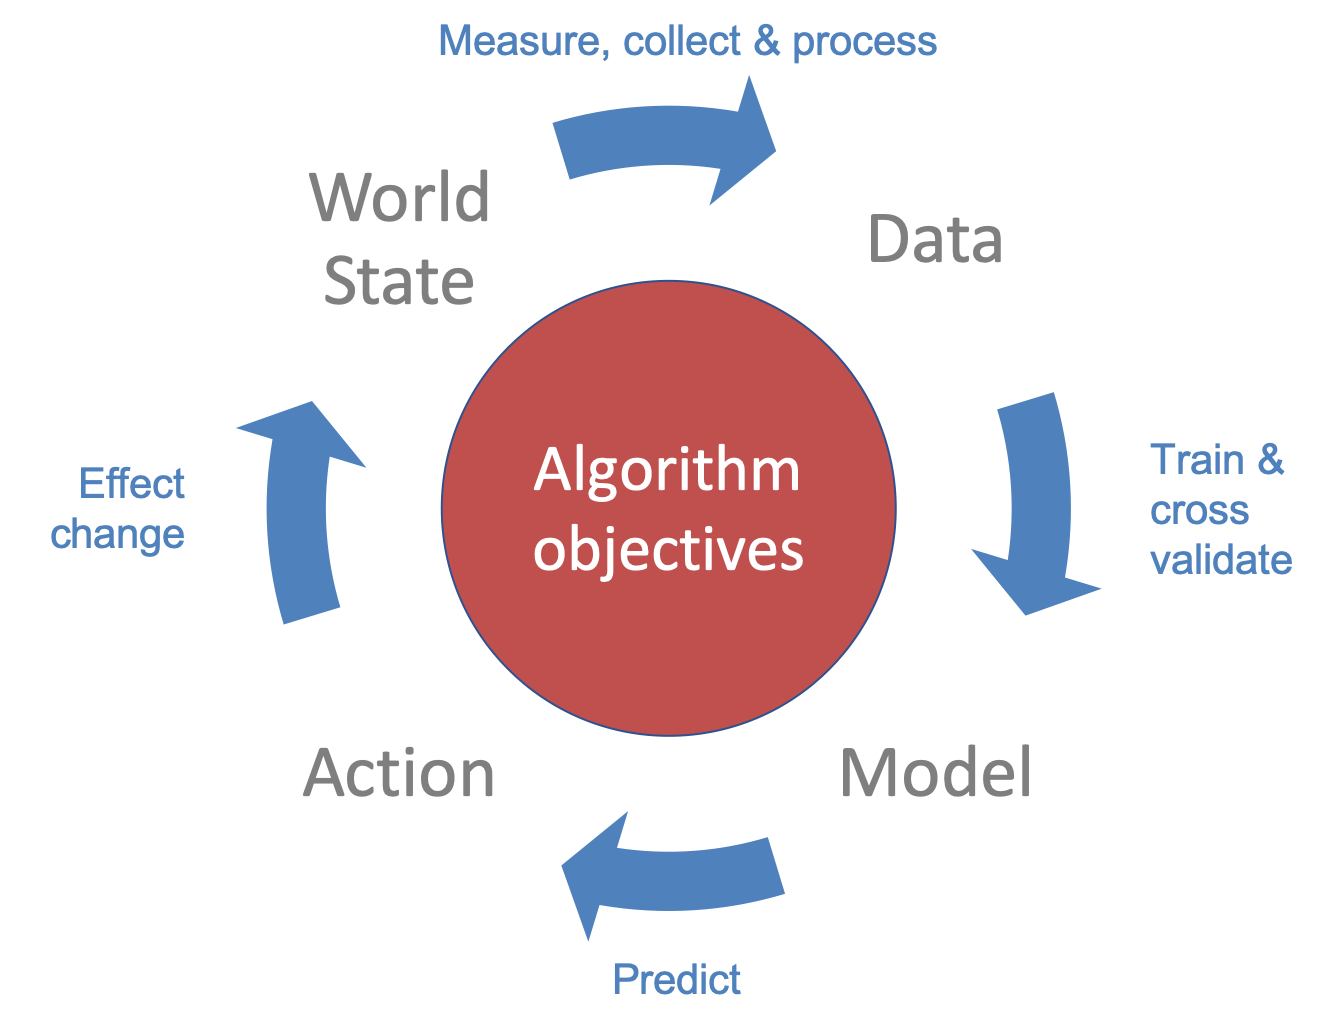
\includegraphics[width=0.9\textwidth]{02_EthicalDevelopment/figures/Fig_MLCycle.png}
\caption{The machine learning cycle}
\label{fig_MLCycle}
\end{figure}

It's important to realise that machine learning solutions can have longterm and compounding effects on the world around us. In this section we analyse the machine learning cycle in a variety of different examples to breakdown the mechanisms that determine the nature and magnitude of the effect. In Figure \ref{fig_MLCycle} we present a high-level depiction of the interaction between a machine learning solution and the real world. At the core of our cycle is some set of objectives. These can be achieved in a myriad of different ways. The translation of these objectives, into a tractable machine learning problem, consists of a series of subjective decisions; what data we train a model on, what events we predict, what features we use, how we clean and process the data, how we evaluate the model and the decision policy are all choices. They determine the model we create, the actions we take and and finally the cycle we end up with.

The most familiar parts of the cycle to most developers of machine learning solutions are on the right hand side; processing data, model selection, training and cross validation and prediction. Each action taken on the basis of our model prediction creates a new world state, which generates new data, which we collect and train or model on, and around it goes again. The actions we take based on our model predictions define how we use the model. The same model used in a different way can result in a very different feedback cycle.

Notice that the world state and data are distinct nodes in in the cycle. Most machine learning models rely on the assumption that the training data is accurate, rich and representative of the population, but this is often not the case. Data is a necessarily subjective representation of the world. The sample may be biased, contain an inadequate collection of features, subjective decisions around how to categorise features into groups, systematic errors or be tainted with prejudice decisions. We may not even be able to measure the true metric we wish to impact. Data collected for one purpose is often reused for another under the assumption that it represents the ground truth when it does not.

Figure \ref{fig_MLCycle} shows the most complete version of the cycle which might not always be the case. In some cases the cycle might be broken. An example might be if one used a dataset to train a model, made decisions based on it and never re-trained the model. Though our model may continually impact the world state, resulting changes are not fed back into the model. The implicit assumption being that the world is static and that taking actions based on the model output does not alter the world state.

%%%%%%%%%%%%%%%%%%%%%%%%%%%%%%%%%%%%%%%%%%%%%%%%%%%%%%%%%%%%%%%%%%%%%%%%%%%%
%%%%%%%%%%%%%%%%%%%%%%%%%%%%%%%%%%%%%%%%%%%%%%%%%%%%%%%%%%%%%%%%%%%%%%%%%%%%
\subsection{Feedback effects}

In cases where the ground truth (target variable) assignment systematically disadvantages certain classes, actions taken based on predictions from models trained on the data can reinforce the bias and even amplify it. Similarly, decisions made on the basis of results derived from machine learning algorithms trained on data that under or over-represents certain classes, can have feedback effects that further skew the representation of those classes in future data. The cycle of training on biased data (which justifies inaccurate beliefs), taking actions in kind, and further generating data that reinforces those biases can become a kind of self-fulfilling prophecy. The good news is that just as we can create pernicious cycles that exaggerate disparities, we can create virtuous ones that have the effect of reducing disparities. Let's take two examples to illustrate the point.

In the United States, predictive policing has been implemented by police departments in several states including California, Washington, South Carolina, Alabama, Arizona, Tennessee, New York and Illinois. Such algorithms use data on the time, location and nature of past crimes, in order to determine how and where to patrol and thus improve the efficiency with which resources are allocated. The aim on the face of it is a noble one - to deter crime from happening - prevention over cure, so to speak. However there is a major flaw with these algorithms. The data used to train these algorithms is not of where crimes occurred (such data does not exist), but rather where there have been previous arrests. A proxy target variable (arrests) is used in absence of available data for the desired target variable (crime). Racial disparities in policing in the US is a well publicised problem (see Figure \ref{fig_drugs}). In 2015, an analysis by The Hamilton Project found that at the state level, Blacks were 6.5 times as Whites to be incarcerated for drug-related crimes\cite{HamProj}. Taking actions based on predictions from an algorithm trained on arrest data will amplify existing disparities between under and over-policed neighbourhoods which correlate with race.
%
\begin{figure}[h!]
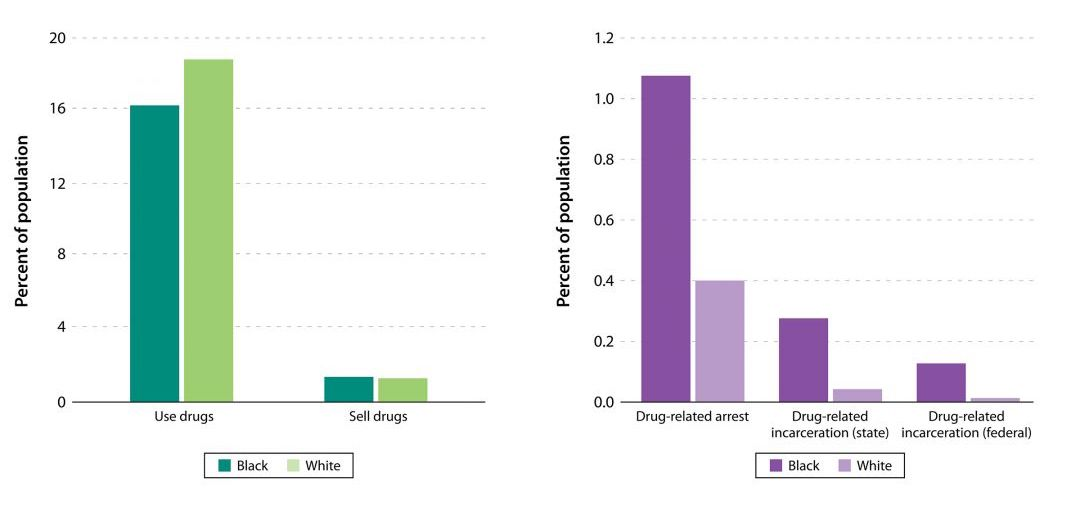
\includegraphics[width=\textwidth]{02_EthicalDevelopment/figures/Fig_RatesDrugUseSaleRace.jpg}
\caption[Rates of drug use and sales compared to criminal justice measures by race.]{Rates of drug use and sales compared to criminal justice measures by race\cite{HamProj}.}
\label{fig_drugs}
\end{figure}

As a comparative example, let's consider car insurance. It is well publicised that car insurance companies discriminate against young male drivers as they are deemed to be at higher risk of being involved in accidents.
%
\begin{lookbox}
\lbtitle{Age discrimination in car insurance}
Take a moment to think about why this is legal or considered fair (despite age and gender being legally protected characteristics in the countries where these insurance companies operate).
\end{lookbox}

Insurance companies act on risk predictions by determining the price of insurance at an individual level - the higher the risk, the more expensive the cost of insurance. What is the feedback effect of this on the data? Of course young men are disadvantaged by having to pay more, but one can see how this pricing structure acts as an incentive to drive safely. It is in the drivers interest to avoid having an accident that would result in an increase in their car insurance premiums. For a high risk driver in particular, an accident could potentially make it prohibitively expensive for them to drive. The feedback effect on the data would be to reduce the disparity in incidents of road traffic accidents among high and low risk individuals.

Along with the difference in the direction of the feedback effects in the examples given above, there is another important distinction to be made in terms of the magnitude of the feedback effect. This is related to how much control the institution making decisions based on the predictions, has over the data. In the predictive policing example the data is entirely controlled by the police department. They decide where to police, who to arrest determining who is and isn't in the data. They produce the training data, in its entirety, as a result of their actions. Consequently, feedback effect of acting on predictions based on the data is strong and capable of shifting the entire distribution of data generated in the future. Insurance companies by comparison, have far less influence over the data (consisting individuals involved in road traffic accidents). Though they can encourage certain driving behaviours through pricing, they do not ultimately determine who does and does not have an accident, even if that insurance company dominates the market. As such, feedback effects of risk-related pricing in car insurance are likely to be less strong in comparison.

%%%%%%%%%%%%%%%%%%%%%%%%%%%%%%%%%%%%%%%%%%%%%%%%%%%%%%%%%%%%%%%%%%%%%%%%%%%%
%%%%%%%%%%%%%%%%%%%%%%%%%%%%%%%%%%%%%%%%%%%%%%%%%%%%%%%%%%%%%%%%%%%%%%%%%%%%
\subsection{Model application and feedback}

A crucial part of responsible model development is understanding and communicating its limitations - what the model can and (perhaps more importantly) cannot be used for. Clearly defining what a model will be used for is an important part of enabling effective and focussed analysis and testing of it. In addition considering the cases for which the model is not suitable and documenting them can prevent models from being used inappropriately.

The idea that the use case for a product, tool or model should be well understood before release; that it should be validated and thoroughly tested for that use case and further that the potential harms caused (even for unintended uses) should be mitigated is not novel. In fact, many industries have safety standards set by a regulatory body that enshrine this idea in law. The motor vehicle industry has a rich history of regulation aimed at reducing risk of death or serious injury from road traffic accidents that continues to evolve today. In the early days, protruding knobs and controls on the dash would impale people in collisions! It was not until the 1960s that seatbelts, collapsing steering columns and head restraints became a requirement. Since then, safety testing and requirements have continued to expand (albeit slowly more recently thanks to reduced funding of regulatory bodies) to including rear brake lights, a variety of impact crash tests, ISOFIX child car seat anchors among others. There are many more such examples across different industries but it is perhaps more instructive to consider an example that involves the use of models.

Derivatives are financial contracts (products) that result in payments dependent on future events. The details, such as amounts and events that lead to payments are described in the contract. For example, a contract that gives the holder the right, but not obligation, to buy 100 units of S\&P 500 (the underlying asset) in a years time (the expiry), at a price fixed today (strike price), is the simplest example of a derivative known as a call option. Derivatives pricing can get complicated quickly as the events which result in payments become more elaborate. In derivatives markets, it is known that models are product specific. A model that is suitable for pricing one financial instrument will not necessarily be appropriate to price another, just because the underlying asset (in our example the S\&P 500) is the same (even though it's the underlying assets behaviour that is being modelled). A derivatives pricing models, for a variety of reasons often only capture limited characteristics of the underlying instrument. For this reason, banks that trade derivatives validate models specifically for the instruments they will be used to price and document their testing. Furthermore they must track their product inventory (along with the model used to price each contract) in order to be able to show that they are not using models to price products for which they have not been approved (validated as part of their internal model review process).

Though machine learning models are not (yet) regulated in the same way, it's easy to see the parallels. Clear consideration of the use case is not just about making sure that the model performs well enough for that use case. How a model is used ultimately determines the actions that are taken off the back of the resulting predictions and thus the nature of the feedback that model has on future data. To illustrate the value of use case specific testing, we return to COMPAS\cite{ProPub2}. The system was not designed to be used in sentencing. Tim Brennan (the co-founder of Northpointe and co-creator of its COMPAS risk scoring system) testified at Paul Zilly's appeal hearing that they ``wanted to stay away from the courts''. Documentation\cite{COMPASguide} for the software (dated 2015) describes it as a risk and needs  assessment and case management system. It talks about it being used ``to inform decisions regarding the placement, supervision and case management of offenders'' and probation officers using the recidivism risk scales to ``triage their case loads'', it does not anywhere discuss its use in sentencing.

Could this model, developed as a case management tool for probation officers be useful in determining the length of an offenders sentence? Napa County, California, uses a similar risk scoring system in the courts. What's interesting is that a Superior Court Judge, who trains other judges in evidence-based sentencing, cautions colleagues in their interpretation of the scores. He outlines a concrete example of where the model falls short. He says ``A guy who has molested a small child every day for a year could still come out as a low risk because he probably has a job. Meanwhile, a drunk guy will look high risk because he’s homeless. These risk factors don’t tell you whether the guy ought to go to prison or not; the risk factors tell you more about what the probation conditions ought to be.”\cite{ProPub2}

So, let's look at the feedback of the model on the data for a variety of different use cases. Propublica's review looked at recidivism risk for more than 10,000 criminal defendants in Broward County, Florida\cite{ProPub3}. Their analysis found the distributions of risk scores for Black and White defendants to be markedly different, with White defendents being more likely to be scored low-risk - see Figure \ref{fig_COMPAS}.
%
\begin{figure}[h!]
\centering
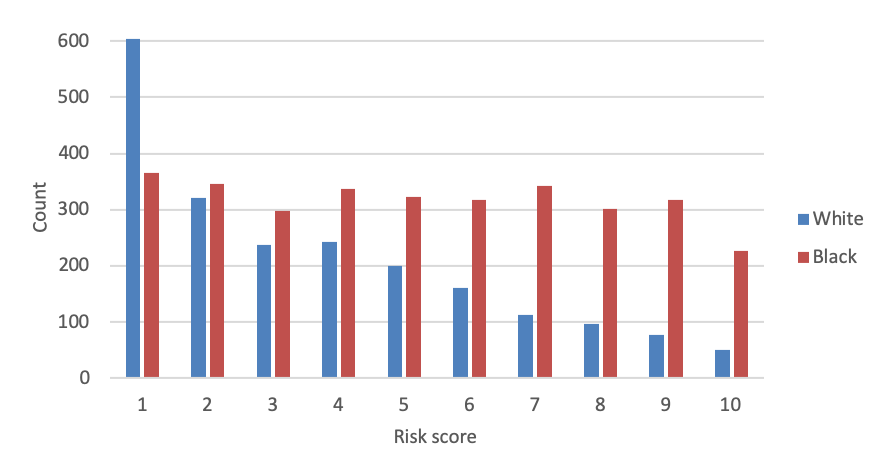
\includegraphics[width=0.85\textwidth]{02_EthicalDevelopment/figures/Fig_Propublica.png}
\caption[Comparison of recidivism risk scores for White and Black defendants.]{Comparison of recidivism risk scores for White and Black defendants\textsuperscript{\cite{ProPub3}}}
\label{fig_COMPAS}
\end{figure}

Comparing predicted recidivism rates for over 7,000 of the defendants with the rate that actually occurred over a two-year period, they found the accuracy of the algorithm in predicting recidivism for Black and White defendants to be similar (59\% for White and 63\% for Black defendants), however the errors revealed a different pattern. They found that Blacks were almost twice as likely as Whites to be labelled as higher risk but not actually re-offend. The errors for White defendants were in the opposite direction; while being more likely to be labelled as low-risk, they more often went on to commit further crimes. See Table \ref{tab_COMPAS}.
%
\begin{table}[h!]
\centering
\caption{COMPAS comparison of risk score errors for White versus Black defendants}
\label{tab_COMPAS}
\vspace{10pt}
\begin{tabular}{|l|r|r|}
\hline
Error type                                 & White  & Black  \\
\hline
\hline
Labelled Higher Risk, But Didn’t Re-Offend & 23.5\% & 44.9\% \\
Labelled Lower Risk, But Did Re-Offend     & 47.7\% & 28.0\% \\
\hline
\end{tabular}
\end{table}
%
Let's assume for a moment that the disparity in recidivism risk between Black and White defendants to be accurate, i.e. that Black defendants do in fact re-offend more often than White defendants, let's consider the feedback effect on the racial disparity for a range of different use cases for the model.

In the courts, when the COMPAS recidivism risk score has been used to determine sentence length as a means to reduce crime - the higher the risk, the longer the sentence. What's the effect on the disparity? Current research suggests that ``The longer and harsher the prison sentence – in terms of less freedom, choice and opportunity for safe, meaningful relationships – the more likely that prisoners’ personalities will be changed in ways that make their reintegration difficult and that increase their risk for re-offending''\cite{BBCFPrison}. The feedback effect of subjecting high-risk defendants to longer sentences would be to further exacerbate the racial disparity, since Black defendants would more often suffer longer sentences resulting in greater difficulty reintegrating into society and increase the liklihood of re-offending upon release. What about reducing crime? What does the research say about that? It is the certainty, rather than severity of punishment that acts as a deterrent to crime\cite{Nagin}. Long-term sentences are particularly ineffective for drug crimes as drug sellers are easily replaced in the community\cite{TheSentProj}. On balance, excessive incarceration has negative consequences for public safety because finite resources spent on prison are diverted from policing, drug treatment, preschool programs, or other interventions that might produce crime-reducing benefits.

Let's consider another use case for recidivism risk scoring. The US has the highest rate of incarceration in the world, at 0.7\% of the population\cite{PrisPolInit}. It's higher than countries with authoritarian governments, those that have recently been locked in civil war and those with murder rates more than twice that in the US. Comparing with countries that have stable democratic governments, the incarceration rate in the US is more than 5 times that of its closest peer - the UK. The US spends \$57 billion a year on housing more than 2.2 million people in prison\cite{BBCFLongSent}, almost half of which are private companies that spend significant sums on lobbying the federal government for policies that would further increase incarceration. Some have advocated for the use of risk scores in sentencing in order to reduce the rate of incarceration, the idea being that if the risk scores are low then defendants can be spared prison time. What would the feedback effect on the observed racial disparity for this use case be? The action is a little different, we `reward' low-risk rather than `punish' high-risk scoring defendants, but the feedback effect would be similar - to increase the existing racial disparity since White defendants will more often be spared prison time.

Finally, what if the software was used as a way to distribute limited rehabilitation resources, allocating them to those defendants that that were deemed to be at the highest risk of re-offending and thus the most in need of help. What would the feedback effect on the racial disparity in this case be? It's easy to see that using the model in this way would reduce the disparity. Of course we have made numerous simplifying assumptions in our analysis of the feedback on the disparity; that rehabilitation consistently reduces the risk of recidivism (regardless of the crime), that recidivism risk is calculated on a long time horizon, that the relationship between sentence length and recidivism is monotonic. Without getting into the weeds, the point here is simply that the same model can have very different feedback cycle if used in a different way. How a model is used is important. The question to ask is, does the action taken on the back of the model serve to push extremes to the centre, or push them further apart? What you have to understand to answer the question, will depend on the specifics of the problem.

%%%%%%%%%%%%%%%%%%%%%%%%%%%%%%%%%%%%%%%%%%%%%%%%%%%%%%%%%%%%%%%%%%%%%%%%%%%%
%%%%%%%%%%%%%%%%%%%%%%%%%%%%%%%%%%%%%%%%%%%%%%%%%%%%%%%%%%%%%%%%%%%%%%%%%%%%
%%%%%%%%%%%%%%%%%%%%%%%%%%%%%%%%%%%%%%%%%%%%%%%%%%%%%%%%%%%%%%%%%%%%%%%%%%%%
\section{Fairness and bias interventions}

We will get in to the details of a range of methods for measuring and mitigating bias and unfairness in the chapters that follow, but first we take a look at where in the machine learning model development workflow these metrics and interventions fit. Figure \ref{fig_Workflow} depicts the model development, deployment and monitoring life cycle at a high level.
%
%\begin{sidewaysfigure}[h!]
\begin{figure}[h!]
\centering
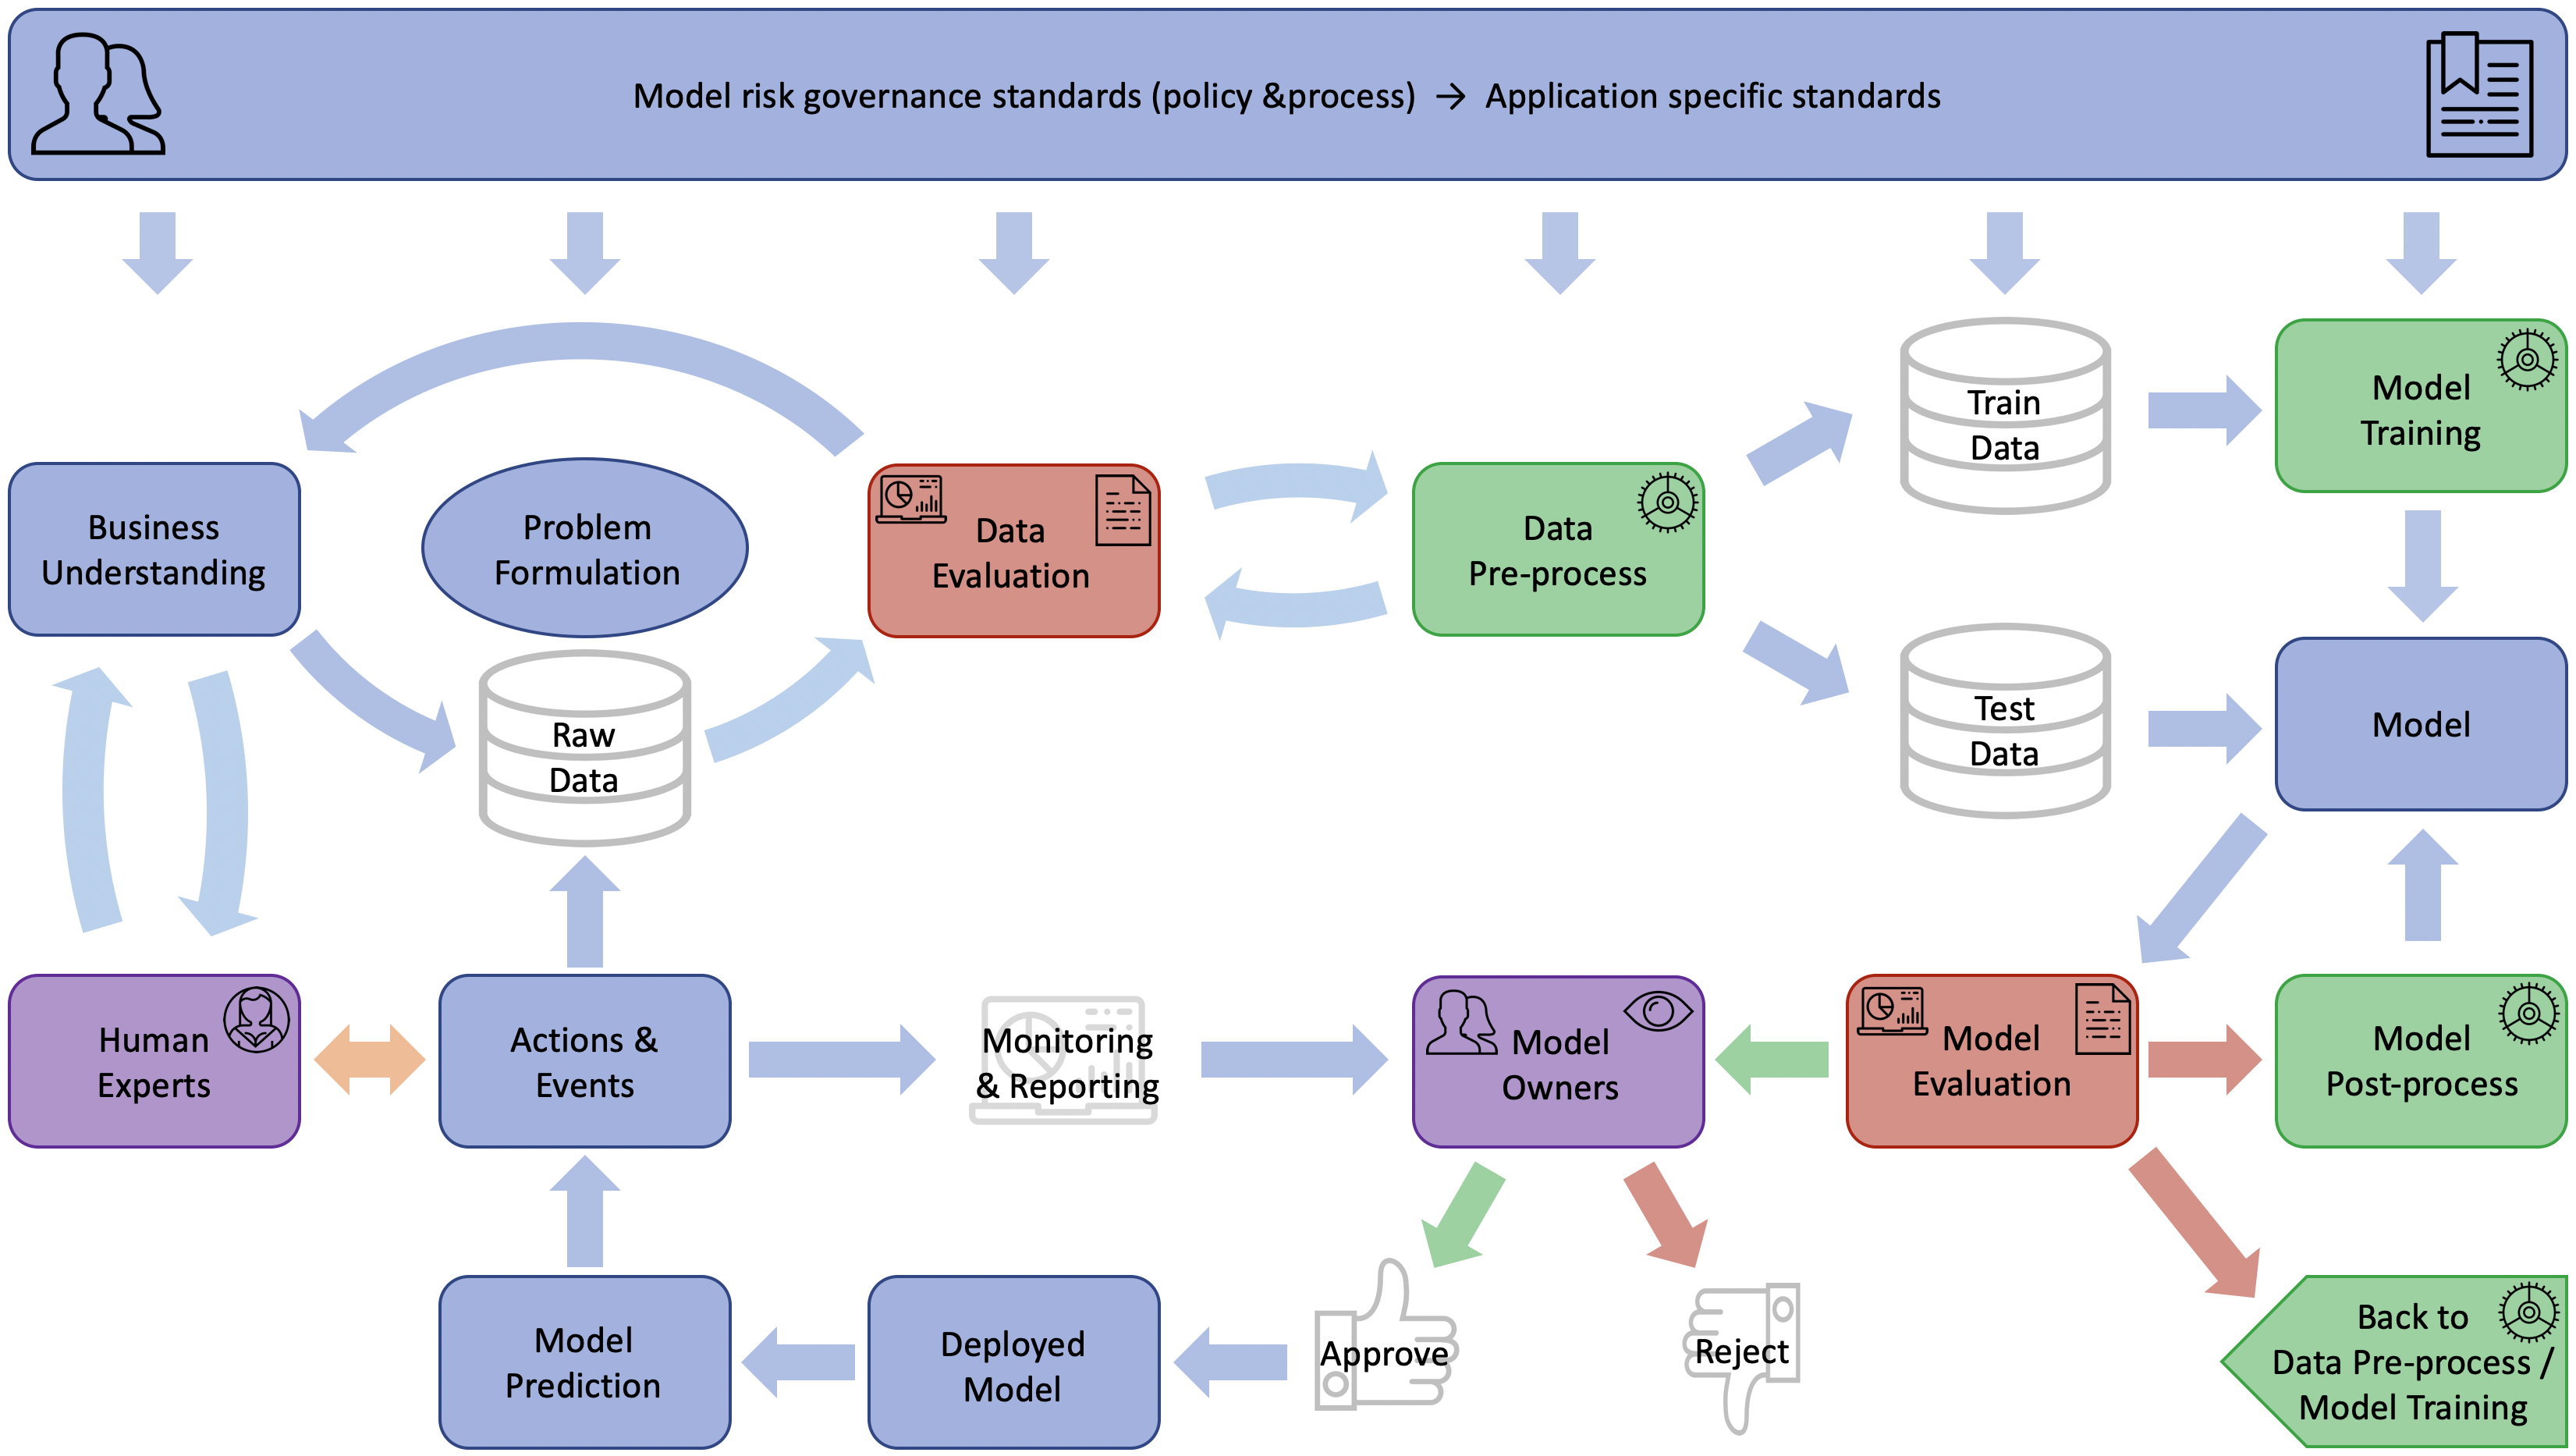
\includegraphics[width=\textwidth]{02_EthicalDevelopment/figures/Fig_Workflow.png}
\caption[Fairness aware machine learning system development, deployment and management workflow.]{Fairness aware machine learning system development, deployment and management workflow. Note, the term `human experts' is context dependent here, in relation to business understanding it is any person with valuable insight or perspective on the product, in relation to decision making it will be a person capable of adjudicating on the evidence to determine the best action.}
\label{fig_Workflow}
\end{figure}
%\end{sidewaysfigure}
%\afterpage{\clearpage}

%%%%%%%%%%%%%%%%%%%%%%%%%%%%%%%%%%%%%%%%%%%%%%%%%%%%%%%%%%%%%%%%%%%%%%%%%%%%
%%%%%%%%%%%%%%%%%%%%%%%%%%%%%%%%%%%%%%%%%%%%%%%%%%%%%%%%%%%%%%%%%%%%%%%%%%%%
\subsection{Metrics}

Bias and fairness metrics are essentially calculated on data. There are two stages at which we'll be interested in measuring bias and or fairness.
%
\paragraph*{Model input} The training data. Node labelled \emph{data evaluation} in Figure \ref{fig_Workflow}.
%
\paragraph*{Model output} The predictions produced by our model. Node labelled \emph{model evaluation} in Figure \ref{fig_Workflow}
\newline

It's worth highlighting at this point that these two need not be the same. That is, bias and fairness metrics calculated on the training data will generally be different to those calculated on the model output for a variety of reasons. By comparing the two, we can evaluate how well the model is replicating the distributions it's trained on, specifically the biases in the data.

%%%%%%%%%%%%%%%%%%%%%%%%%%%%%%%%%%%%%%%%%%%%%%%%%%%%%%%%%%%%%%%%%%%%%%%%%%%%
%%%%%%%%%%%%%%%%%%%%%%%%%%%%%%%%%%%%%%%%%%%%%%%%%%%%%%%%%%%%%%%%%%%%%%%%%%%%
\subsection{Mitigation techniques}

There are essentially three stages at which one can intervene to mitigate bias when developing a machine learning model and we categorise them accordingly:
%
\paragraph*{Pre-processing} techniques modify the historical data on which the model is trained, the idea being that fair/unbiased data will result in a fair/unbiased model once trained. Node labelled \emph{data pre-process} in Figure \ref{fig_Workflow}.
%
\paragraph*{In-processing} techniques alter the training process or objective in order to create model with fairer/less biased predictions. Node labelled \emph{model training} in Figure \ref{fig_Workflow}.
%
\paragraph*{Post-processing} techniques take a trained model and modify the output such that the resulting predictions are fairer/less biased. Node labelled \emph{model post-process} in Figure \ref{fig_Workflow}.

%%%%%%%%%%%%%%%%%%%%%%%%%%%%%%%%%%%%%%%%%%%%%%%%%%%%%%%%%%%%%%%%%%%%%%%%%%%%
%%%%%%%%%%%%%%%%%%%%%%%%%%%%%%%%%%%%%%%%%%%%%%%%%%%%%%%%%%%%%%%%%%%%%%%%%%%%
\subsection{Can a model be biased?}

A common belief shared by many well known and respected professional machine learning scholars and practitioners is that bias comes from the data not the model. We've spoken about numerous examples of biased models in this book already. So what do people mean when they say this? In more theoretical disciplines a model is interpreted as being the parametric form (so that different values of the parameters don't change the model, for example, the term \emph{linear model} describes a family of models). More practical disciplines view a model more as a black box - provided with input, the model returns output (if the parameters change, the output changes and so must the model). From a practical perspective then it's clear that a model can discriminate since if the data discriminates so does the model (assuming the model fits the data reasonably well).

The notion that bias is an artefact of data, rather than a model is at best counterproductive and at worst misleading. It implies that models and data are independent when they are not. Model development is an iterative process. The modelling choices we make will depend on the data, and model results will in turn influence our choices regarding the training data. Treating the data and model as independent entities diminishes the responsibility of model developers in addressing the problem of biased and unfair algorithms and ignores the very practical nature of developing models to solve real world problems. If we are developing a model as a means to understand the world then it may make sense for utility to be our sole objective because the goal is simply to find out how well the model fits observations. For an application that will be used to make predictions that have an impact in the real world, the objectives should extend beyond utility to other metrics. Those other metrics will depend on the problem, in part 2 of this book we'll explore a range of metrics that measure notions such as fairness and diversity.

%%%%%%%%%%%%%%%%%%%%%%%%%%%%%%%%%%%%%%%%%%%%%%%%%%%%%%%%%%%%%%%%%%%%%%%%%%%%
%%%%%%%%%%%%%%%%%%%%%%%%%%%%%%%%%%%%%%%%%%%%%%%%%%%%%%%%%%%%%%%%%%%%%%%%%%%%
%%%%%%%%%%%%%%%%%%%%%%%%%%%%%%%%%%%%%%%%%%%%%%%%%%%%%%%%%%%%%%%%%%%%%%%%%%%%
\section{Common causes of bias}

There are many ways in which machine learning solutions can produce biased predictions. In this section we present a taxonomy of common causes with examples. In addition we relate the causes in the taxonomy to the corresponding stages of the model development and deployment life cycle so that it may be used as a reference when designing machine learning solutions in order to avoid common pitfalls. We follow the taxonomy described in the excellent paper by d'Alessandro et. al.\cite{}, giving additional examples where valuable. Table \ref{tab_Taxonomy} summarises the taxonomy of common causes of bias in a machine learning system.
%
\begin{table}[h!]
\caption[Taxonomy of common causes of bias in machine learning models.]{Taxonomy of common causes of bias in machine learning models\cite{ConsClfn}.}
\label{tab_Taxonomy}
\centering
\vspace{10pt}
\begin{tabular}{|l|l|l|l|}
\hline
Component & Root Cause          & Issue Type      & Issue Description                                         \\
\hline
\hline
Model     & Data Issue          & \multicolumn{2}{c|}{Discrimination in data}                                 \\
\cline{3-4}
Issue     &                     & Sample Bias     & Under-representation of protected class                   \\
\cline{4-4}
          &                     &                 & Over-representation of protected class                    \\
\cline{3-4}
          &                     & \multicolumn{2}{c|}{Low support}                                            \\
\cline{2-4}
          & Misspecification    & Target variable & Target variable subjectivity                              \\
\cline{4-4}
          &                     &                 & Proxy target variable learning                            \\
\cline{4-4}
          &                     &                 & Heterogeneous target variable                             \\
\cline{3-4}
          &                     & Features        & Inclusion of protected features without control variables \\
\cline{4-4}
          &                     &                 & Inclusion of protected feature proxies (redlining)        \\
\cline{3-4}
          &                     & Cost function   & Failure to specify asymmetric error costs                 \\
\cline{4-4}
          &                     &                 & Omitted discrimination penalties                          \\
\hline
\hline
System /  & Failure to validate & \multicolumn{2}{c|}{Data appropriateness and preparation}                   \\
\cline{3-4}
Process   &                     & \multicolumn{2}{c|}{Modelling approach, implementation and evaluation}      \\
\cline{2-4}
Issue     & Failure to monitor  & \multicolumn{2}{c|}{Poor feedback loop}                                     \\
\cline{2-4}
          & \multicolumn{3}{c|}{Non-deference to human expert}                                                \\
\hline
\end{tabular}
\end{table}

Figure \ref{fig_Taxonomy} shows the causes of bias in the context of the model development and deployment workflow, indicating both the stages of the workflow to which they relate along with their categorisation within the taxonomy.
%
%\begin{sidewaysfigure}[h!]
\begin{figure}[h!]
\centering
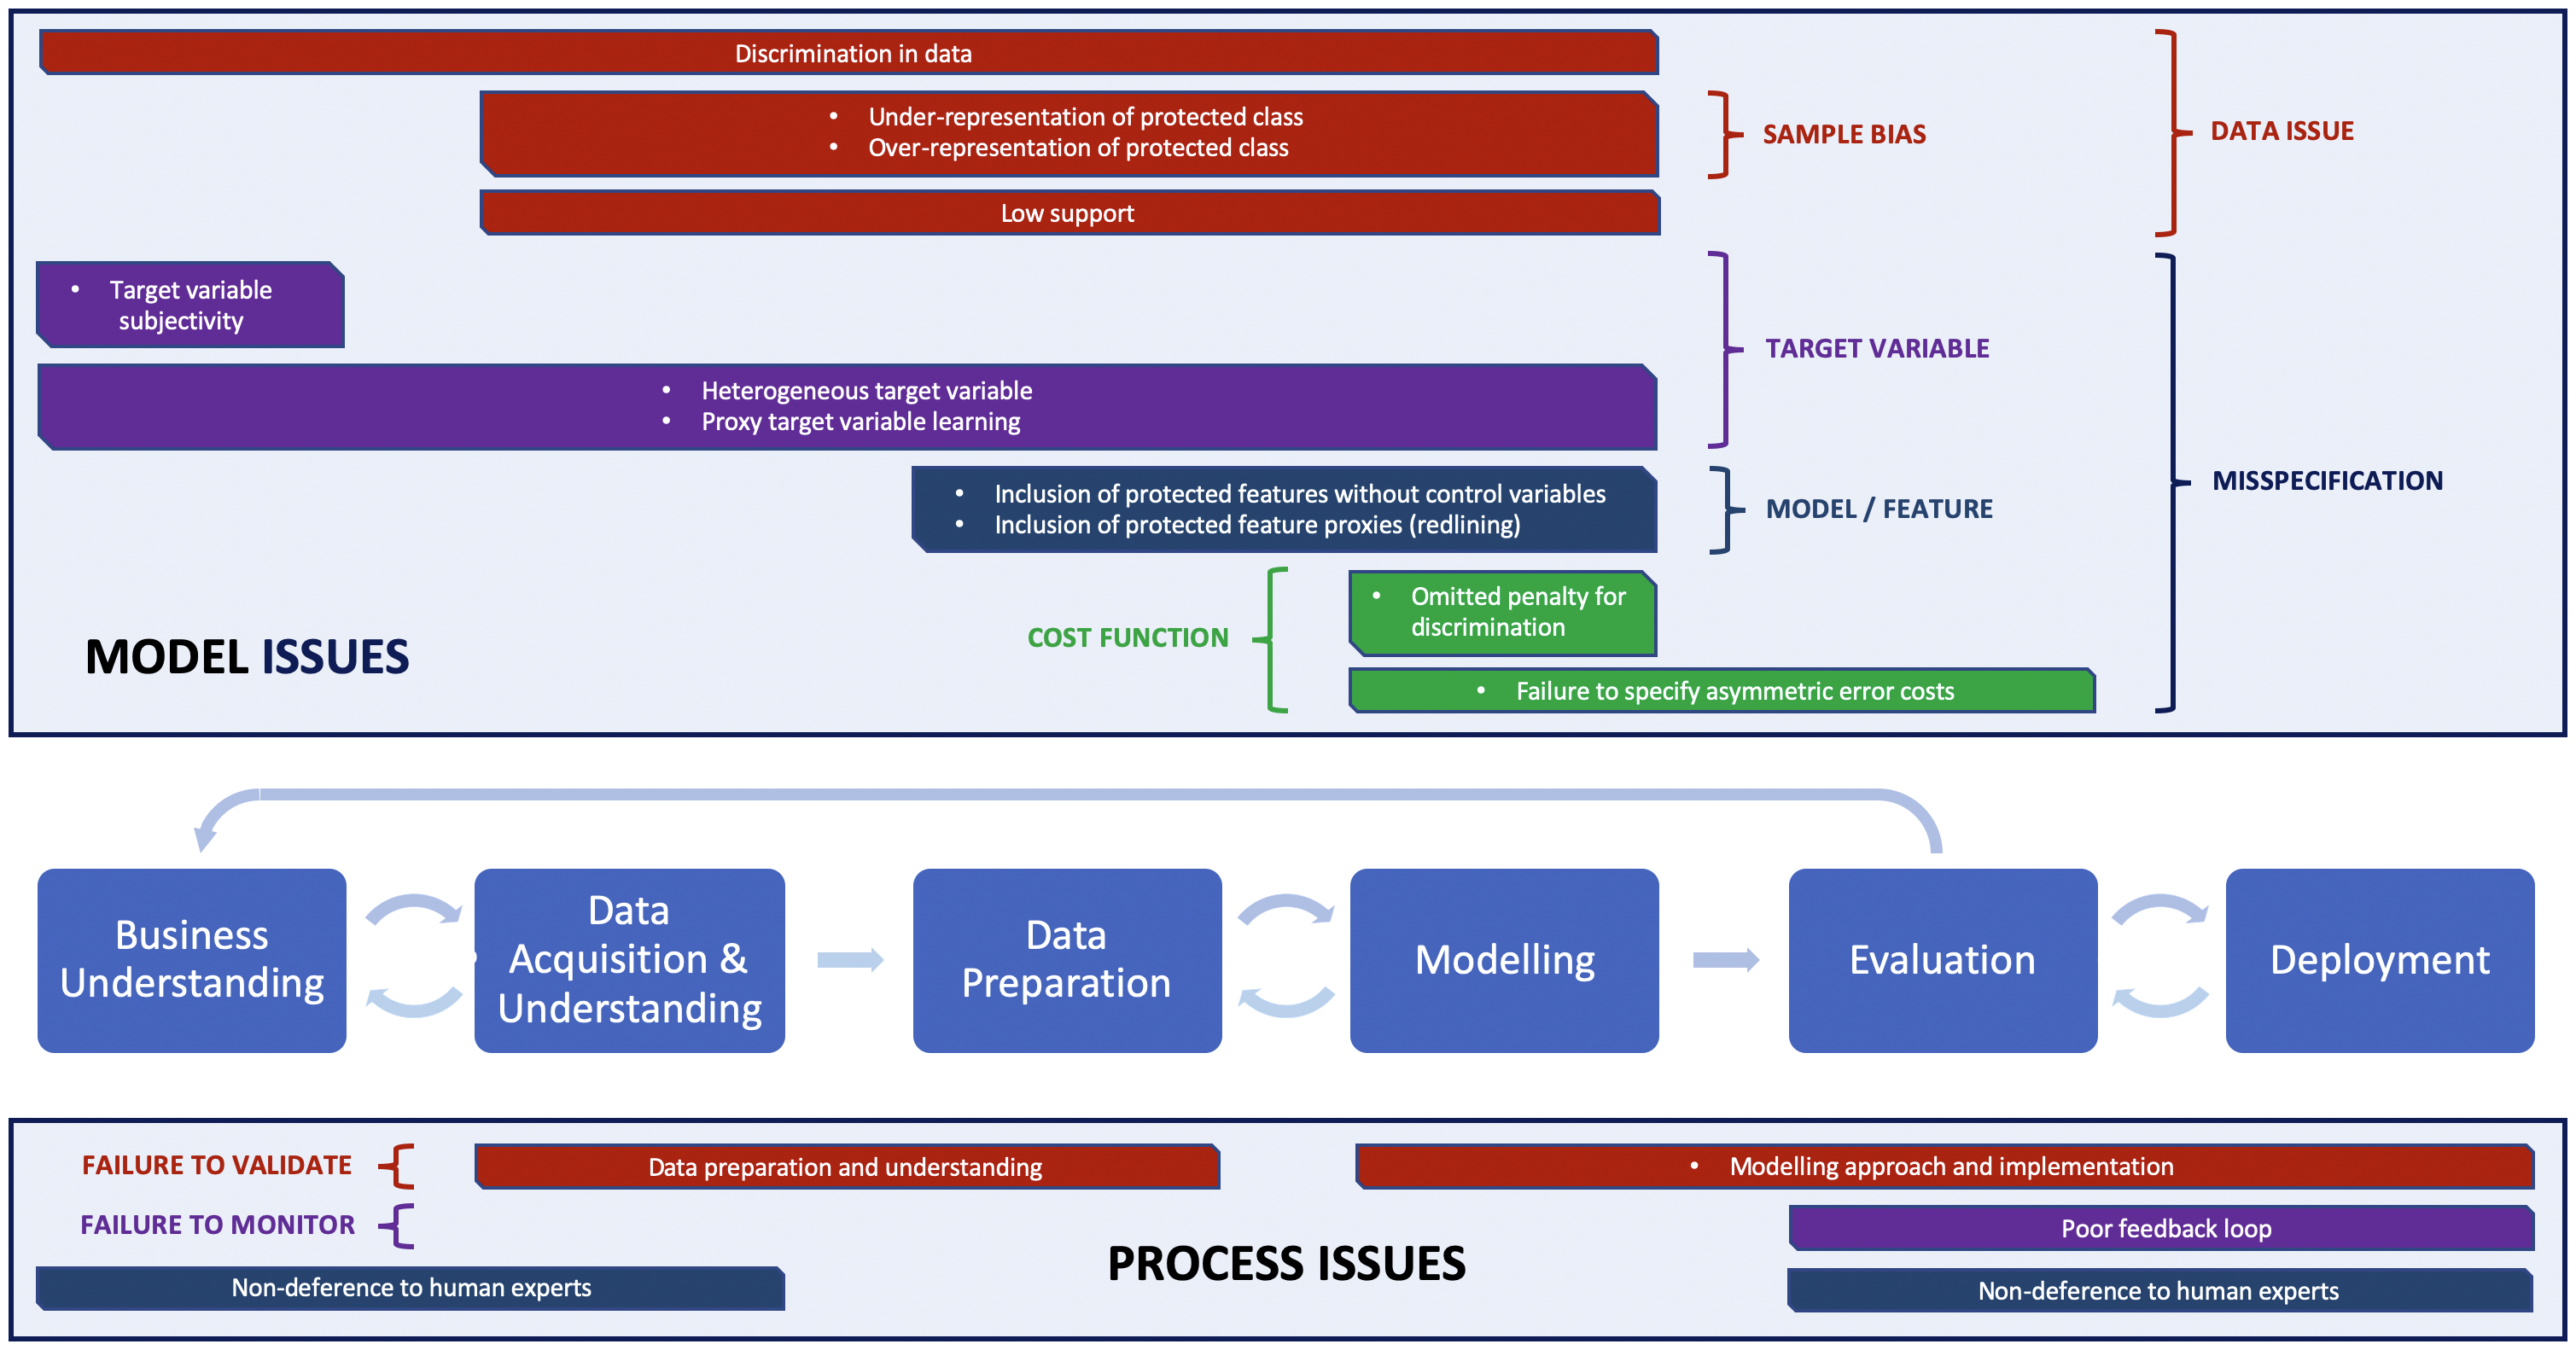
\includegraphics[width=\textwidth]{02_EthicalDevelopment/figures/Fig_Taxonomy.png}
\caption[Taxonomy of common causes of bias in machine learning models.]{Taxonomy of common causes of bias in machine learning models together with the stages of the model development and deployment life cycle they relate to.}
\label{fig_Taxonomy}
\end{figure}
%\end{sidewaysfigure}
%\afterpage{\clearpage}
%
The central row of Figure \ref{fig_Taxonomy} shows a flow diagram representing the model development and deployment life cycle (at a higher level than that shown in Figure \ref{fig_Workflow}). For the purposes of the taxonomy, we distinguish the machine learning model from the larger machine learning system, of which it is a component.
%
\begin{enumerate}[leftmargin=*]
\item \textbf{The machine learning model} is defined as the function mapping $f$ from features $(\boldsymbol{X}, \boldsymbol{Z})$ to predictions $\hat{Y}$.
\item \textbf{The machine learning system} includes the wider infrastructure, processes and policies around development, deployment and monitoring of the model.
\end{enumerate}
%
From Table \ref{tab_Taxonomy} we can see that we categorise the causes of bias as one of two types, those that relate directly to the model (shown in the box above the flow diagram in Figure \ref{fig_Taxonomy}) and those that arise as a result of failures in the model development and deployment process (shown in the box below the flow diagram in \ref{fig_Taxonomy}). The causes of bias within each of these categories are further displayed in boxes, the width of which indicate the stages of the workflow to which they relate. Curly brackets are used to indicate the categorisation of the cause in the taxonomy. In the sections that follow we go through the taxonomy of common causes of bias and provide examples.

%%%%%%%%%%%%%%%%%%%%%%%%%%%%%%%%%%%%%%%%%%%%%%%%%%%%%%%%%%%%%%%%%%%%%%%%%%%%
%%%%%%%%%%%%%%%%%%%%%%%%%%%%%%%%%%%%%%%%%%%%%%%%%%%%%%%%%%%%%%%%%%%%%%%%%%%%
\subsection{Modelling issues}

In this section we discuss common causes of discrimination that relate directly to the model. We categorise these as originating from one of two sources:
\begin{enumerate}[leftmargin=*]
\item \textbf{Data issues} refer to bias that arises as a direct result of issues with the data
\item \textbf{Misspecification} refers to issues relating to misspecification of the underlying problem in the modelling of it.
\end{enumerate}
The latter is an extension of the notion of model misspecification in statistics where the functional form of a model does not adequately reflect reality.

%%%%%%%%%%%%%%%%%%%%%%%%%%%%%%%%%%%%%%%%%%%%%%%%%%%%%%%%%%%%%%%%%%%%%%%%%%%%
\subsubsection*{Data issues}

Within data issues we organise potential sources of bias into three types
\begin{enumerate}
\item \textbf{Discrimination in data:} Disparities between protected classes, in either outcomes or accuracy and completeness are observed in the data.
\item \textbf{Sample Bias:} The data is not representative of the population - protected classes are under or over-represented.
\item \textbf{Low support:} Minority classes naturally have fewer data points to train on.
\end{enumerate}

%%%%%%%%%%%%%%%%%%%%%%%%%%%%%%%%%%%%%%%%%%%%%%%%%%%%%%%%%%%%%%%%%%%%%%%%%%%%
\paragraph*{1. Discrimination in data}

The most obvious way that bias can enter a machine learning model is through the data it is trained on. Discrimination against protected classes is a part of our history and a reality of our society and the data reflects this. One of the goals of training is to in fact replicate the distribution of the data it is trained on. If the training data contains biases we naturally would expect these to propagate through to the predictions of the resulting algorithm. The most obvious way in which this is seen is through a disparity in outcomes between different subgroups of the population. Take medical data where racial and gender disparities in diagnosis and treatment are well publicised as the \emph{health gap}. In particular, there is a growing body of research across the US and Europe that exposes systematic undertreatment and misdiagnosis of pain in women and Black patients.
%
\begin{itemize}[leftmargin=*]
%
\item A 1990 study that looked at medication administered to postoperative coronary artery bypass graft patients differed significantly by gender. Men were more frequently administered pain medication compared to female patients and that female patients were more frequently administered sedative medication\cite{CalderoneSexRoles}.
%
\item A 2008 study found that women were less likely to receive opioid analgesia than men when reporting acute abdominal pain at an emergency department\cite{SexAnalgesic}.
%
\item A 2001 paper surveys extensive research showing that despite evidence that women report more severe, frequent and longer duration of pain than men, they are treated less aggressively for it\cite{GirlPain}.
%
\item Research in the US in 2012 showed that Black patients are 22\% less likely than Whites to be given pain medication and 29\% less likely that Whites to be treated with opioids (despite prescription drug abuse being more prevalent among White Americans).
%
\item A study in 2015 showed that this disparity in pain treatment extended to children with White children being three times more likely to be treated with opioids for appendicitis.
%
\item In a 2016 US study, 200 medical students and residents were given a series of statements about biological differences between White and Black people (such as ``Black people’s skin is thicker than White people’s skin'') and asked to say whether they were true or false. Half the respondents marked false statements as true. Later when given case studies for Black and White patients reporting pain, those participants that held those beliefs rated the Black persons pain lower and made less accurate treatment recommendations\cite{RacialBiasPain}.
%
\end{itemize}

A more subtle way in which discrimination can manifest in data is where the accuracy and completeness of records are correlated to sensitive features. This can happen for example, where there are geographic disparities in services provided by institutions (which tend to be correlated with race) or where institutions systematically fail to produce accurate and timely records for protected groups. A good example of the latter is again provided by medical data. Misdiagnosis leads to longer lags between the reporting of symptoms and accurate diagnosis. Given the above we might expect greater delays in accurate diagnosis for protected classes. A study of 12,000 rare disease patients across Europe in 2009 which found significant diagnosis delays for women compared to men\cite{EU12K}; for example 12 compared to 20 months for Crohn's disease (despite being more common among women) and 16 compared to 4 years for Ehlers-Danlos syndrome. Systematic delays in diagnosis for protected groups mean that for any given snapshot in time, the medical records for more frequently misdiagnosed groups are less accurate.

%%%%%%%%%%%%%%%%%%%%%%%%%%%%%%%%%%%%%%%%%%%%%%%%%%%%%%%%%%%%%%%%%%%%%%%%%%%%
\paragraph*{2. Sample Bias}

Another, way in which the training data can result in biased predictions is where there is an imbalance in the prevalence of classes of sensitive features in the training data. All too often training data is assumed to be representative of the population that the model will serve, where it is not. Both under and over representation can be disadvantageous.

Under-represented classes are exposed to higher error rates a problem which arises as a result of `low support', that is a smaller pool of data points to train the model on. Let's briefly examine why this might happen. In training we are trying to find the set of model parameters which minimizes some aggregate measure of model error on training data (the `cost' function). If the contribution to the cost from majority classes dominates (which it will without intervention) the algorithm is naturally incentivised to focus learning characteristics of majority classes as a means of reducing the cost faster. Majority classes being more richly represented by the data results in the model being better able to generalize to them.

In 2017, Joy Buolamwini and Timnit Gebru conducted a seminal study Gender Shades\cite{GenderShades} which found that systems sold by IBM, Microsoft, and Face++ had as high as a 34.4\% accuracy gap in gender classification, between lighter-skinned males and darker-skinned females. Error rates on lighter-skinned males did not exceed 1\%. While we can't be sure without seeing the data these algorithms were trained on, a lack of adequate representation of darker-skinned females in the training data is more than likely at least a contributing factor to such disproportionate error rates. Dataset bias (an over reliance on a single dataset for testing and benchmarking), is a well known issue in computer vision tasks.

One of the drivers behind big data initiatives is the plummeting cost of collection and storage data. Companies and institutions are able to train models that better target individuals, reducing costs and boosting profits. However, often data collection methods fail to adequately represent historically disadvantaged classes of people who are often less engaged in certain data generating ecosystems. A good example of this, given by Barocas \& Selbst\cite{BarocasSelbst} is that of the phone app \href{https://www.boston.gov/transportation/street-bump}{Street Bump}, which was developed by the City of Boston to reduce the cost and time taken to find (and consequently repair) pot holes. The app uses data generated by the accelerometers and GPS of Boston residents' smart phones as they drive. Once a pothole is located it is automatically added to the city's system to schedule a repair. One can see easily see how this method of data collection might fail to adequately capture data from poorer neighbourhoods, where car and smart phone ownership are less prevalent; neighbourhoods which probably correlate with race and are already likely to suffer from lack of investment.

Over-representation of classes can also result in bias through increased scrutiny. Predictive policing discussed earlier provides an example of this. But in practice any process (algorithmic or otherwise) which seeks to identify negative behaviour in which disproportionate resource is allocated to some subgroup will result in disproportionately more instances of that negative behaviour being observed among members of that group. The result is induced correlation in the data between the negative behaviour and over-scrutinised class even if in reality there is none. If an algorithm that seeks to identify negative behaviours is used to determine where to allocate resource to identifying those behaviours in the future, an implicit assumption is made that where no observation was made the negative behaviour did not occur. If observations are not uniformly distributed across the population, the result will be a pernicious cycle that continually amplifies the association between the negative behaviour and members of the over-scrutinised class.

%%%%%%%%%%%%%%%%%%%%%%%%%%%%%%%%%%%%%%%%%%%%%%%%%%%%%%%%%%%%%%%%%%%%%%%%%%%%
\paragraph*{3. Low support}

It is worth briefly mentioning that the problem of low-support need not be a result of under-representation of classes. This is a particular problem for individuals belonging to multiple disadvantaged classes for example Black women.

%%%%%%%%%%%%%%%%%%%%%%%%%%%%%%%%%%%%%%%%%%%%%%%%%%%%%%%%%%%%%%%%%%%%%%%%%%%%
\subsubsection*{Misspecification}

We categorise mispecification as one of three types, based on which aspect of the modelling they relate to
\begin{enumerate}
\item \textbf{Target variable:} the events our model predicts
\item \textbf{Features:} the features we use in our model
\item \textbf{Cost function:} how we evaluate our model in training
\end{enumerate}

%%%%%%%%%%%%%%%%%%%%%%%%%%%%%%%%%%%%%%%%%%%%%%%%%%%%%%%%%%%%%%%%%%%%%%%%%%%%
\paragraph*{1. Target variable}

We discuss three common issues related to the target variable definition:
%
\begin{itemize}
\item Target variable subjectivity
\item Proxy target variable learning
\item Heterogeneous target variable
\end{itemize}

One of the challenges in developing a machine learning is the translation of the underlying problem by definition of a target variable - something which can be observed, measured and recorded accurately. While there are relatively uncontentious examples that machine learning solutions lend themselves well to (spam detection in email or on-base and slugging percentage for player valuation in Major League Baseball). Often however, this translation is non-trivial and rather subjective. It requires the model developer to interpret some problem and translate objectives and requirements into a target variable that can be measured or is accessible in order to set up a tractable machine learning problem.

For the purpose of illustration, consider the problem of determining which candidates from a pool would make `good' employees. How do we determine what a good employee looks like? What might our target variable be? Do they produce results faster? Do they stay with the company longer? Do they take less annual leave? Perhaps they have better annual performance ratings? Each of the above variables would likely exhibit correlations with protected classes that would result in different kinds of biases infiltrating our algorithm. The data might show for example that men tend to stay with the company longer but this might simply be because the workplace is more hostile towards women and bear no relation to how good the employee actually is.

Of course one of the problems in the above example (in addition to the subjectivity in the choice of target variable) is that, like with the predictive policing example, data on the variable we want doesn't really exist so we use a proxy that we believe to be correlated with the variable we wish to affect. In 2018, Amazon was forced to scrap a recruitment tool it spent four years developing. The algorithm rated resumes of potential employees and was trained on 10 years worth of resumes submitted by job applicants. The exact details of the algorithm were not publicised but based on what we know about the training data, it is likely that the proxy variable they used was some measure of how the candidates had performed in the hiring process, and potentially beyond, in the past.

Another common issue is the use of a heterogeneous target variable, where a range of different events are coarsely grouped into a single outcome. This might happen for example where the event of particular interest is rare and by including more events in the target the predictive accuracy of the model increases as it has more data to learn from. D'Alessandro et. al\cite{ConsClfn} provide a useful example in predictive policing where the model developer is initially interested in predicting violent crime but ends up incorporating petty crimes (which happen much more frequently) in the target variable in pursuit of a more accurate model.

%%%%%%%%%%%%%%%%%%%%%%%%%%%%%%%%%%%%%%%%%%%%%%%%%%%%%%%%%%%%%%%%%%%%%%%%%%%%
\paragraph*{2. Features}

We discuss two issues related to feature selection:
%
\begin{enumerate}
\item Inclusion of protected features without control variables
\item Inclusion of protected feature proxies (redlining)
\end{enumerate}

In an ideal world we would train a machine learning model on a sufficiently large dataset consisting of a rich set of features that actually influence the target variable rather than simply being correlated to it. More often than not, the reality is rather different. Comprehensive data can be expensive and difficult to collect. Factors that influence the target variable might not be easily measured or be measurable at all, while data containing more erroneous indicators might simply be cheaper to obtain or more readily available. This is a common way in which bias against protected classes can enter our model. 

We discuss two cases. In the first we include a protected feature because it appears to be predictive of the target variable. Of course using protected characteristic when building a model would invariably come with disparate treatment liability so is not a problem one is typically faced with but we take this opportunity to recall the importance of controlling for confounding variables, in drawing conclusions about relationships between features from observational data (see section \ref{sec_SimpsParadox}).

The second (more common) case is one where we do not use protected features in the model but use features which are predictive of them. Take another example in the context of hiring. Historically employers have taken the reputation of the university that applicants graduated from as a strong indicator of the calibre of the candidate. But many of the most reputable universities have very low rates of non-White/Asian students in attendance. A hiring process which is strongly influenced by the university from which the applicant graduated, can erroneously disadvantage racial groups that are less likely to have attended them. While the university an applicant graduated from, might correlate to some degree with success in a particular role it is not in itself the driver. An algorithm that directly takes into account the skills and competencies required for the role would be more predictive and simultaneously less biased. Given the cost of collecting comprehensive data, one might argue that higher error rates for some classes would be financially justified (rational prejudice).

%%%%%%%%%%%%%%%%%%%%%%%%%%%%%%%%%%%%%%%%%%%%%%%%%%%%%%%%%%%%%%%%%%%%%%%%%%%%
\paragraph*{3. Cost function}

We discuss two issues related to the cost function specification:
%
\begin{enumerate}
\item Failure to specify asymmetric error costs
\item Omitted discrimination penalties
\end{enumerate}

A critical consideration in how we specify our model is the cost function.  It is how we evaluate our model in training and essentially determines the model (parameters) we end up with. The cost function can be interpreted as an expression of our model objectives and so provides a natural route to addressing discrimination concerns. A common failure in the design of classification models is proper accounting of the costs of the different types of classification errors (false negative versus false positives). If the harm caused by the different types of misclassification are asymmetric, the cost matrix should reflect this asymmetry.

More broadly (for both regression and classification), it is important to consider the contribution from each sample in the training data to the cost function in training. Upsampling (or simply upweighting, depending on the learning algorithm you are using) is a valuable tool to keep in mind and can alleviate a number of the issues discussed above, that are common sources of bias. Let's take the issue of low support. By upsampling minority classes, one can increase the importance of reducing errors for those data points, relative to other more abundant classes, during learning. Though it's worth noting that it cannot resolve issues relating to a lack of richness of representation for classes with low support. Another case in which upsampling can help is that discussed in relation to definition of a heterogeneous target variable. By upsampling data points that correspond to the primary event of interest (violent crime in the example we discussed above), one can again increase the importance of the model fitting to those data points.

For an algorithm that solves a problem in a regulated domain, it would make sense for the absence of discrimination to be a model objective along with utility. This can be achieved by use of a penalty term in the cost function which relates to discrimination in the resulting predictions (just as we have terms that relate to the error or overfitting). Essentially the idea is similar to that of regularisation to avoid overfitting. We introduce an additional hyper-parameter to tune, which represents the strength of the penalty for discrimination in our cost. We will discuss this and upsampling in more detail when we discuss bias mitigation techniques, in part three of the book.

%%%%%%%%%%%%%%%%%%%%%%%%%%%%%%%%%%%%%%%%%%%%%%%%%%%%%%%%%%%%%%%%%%%%%%%%%%%%
%%%%%%%%%%%%%%%%%%%%%%%%%%%%%%%%%%%%%%%%%%%%%%%%%%%%%%%%%%%%%%%%%%%%%%%%%%%%
\subsection{System / process issues}

In this section we discuss failures that relate to the larger machine learning system (rather than more directly to the model). Any institution (no matter how big or small) that uses models in a setting where there are real world consequences of the model being wrong should have processes in place to ensure the risks are assessed, understood and mitigated. We talk about the kinds of processes that form part of a responsible development and deployment in the section that follows but cover them at a high level here for completeness. We consider three ways in which process interventions play a critical role in avoiding bias in machine learning systems.
\begin{enumerate}
\item \textbf{Validation} and testing of the approach, data and model pre-deployment
\item \textbf{Monitoring} of the model post-deployment
\item \textbf{Keeping human experts in the loop} in development and post-deployment
\end{enumerate}

%%%%%%%%%%%%%%%%%%%%%%%%%%%%%%%%%%%%%%%%%%%%%%%%%%%%%%%%%%%%%%%%%%%%%%%%%%%%
\subsubsection*{1. Failure to validate}

We discuss two important aspects of the modelling which should be appropriately validated pre-deployment
%
\begin{enumerate}
\item Data appropriateness and preparation
\item Modelling approach, implementation and evaluation
\end{enumerate}

A common failure that results in biased algorithms is inadequate review and validation of a machine learning systems pre-deployment. Testing for discrimination should be built into the model/product development process. Interpretation and translation of ethical standards into data/model/product requirements, consideration of the resulting machine learning cycle and determining appropriate metrics should be an integral part of the problem formulation and solution design.

An assessment should be made with regards to how appropriate the data is for the model use case. Understanding the provenance of the data (who collected it, how it was collected and for what purpose) is important. Is it representative of the population the model built on it intends to serve? Exploratory data analysis (EDA) should include understanding if there is bias and or discrimination in the data. In particular understanding how is the target variable distributed for different subgroups of the population and what the nature of the resulting machine learning cycle might be for the intended and unintended use cases. Is there strong correlation between protected features and other variables? Data preparation methods should also be analysed for potential biases they may introduce. Methods for measuring and mitigating bias as part of data preparation may be used and should also be analysed during development and model review.

The process of testing and analysing model output for performance should also include corresponding analysis for discrimination and fairness. How are predictions and errors distributed for different subgroups of the population? How does the model output distribution differ from the training data? What are the limitations of the model? What should it not be used for and why? Again methods for measuring and mitigating bias may also be used and should be properly analysed.

%%%%%%%%%%%%%%%%%%%%%%%%%%%%%%%%%%%%%%%%%%%%%%%%%%%%%%%%%%%%%%%%%%%%%%%%%%%%
\subsubsection*{2. Failure to monitor}

Post-deployment monitoring is an important part of responsible model development and deployment. Analysis should not stop once the model is deployed. Decisions on what to monitor and necessary feedback mechanisms should be determined during development. It's important to understand if the model is performing in line with expectations (based on pre-deployment testing and analysis). Are there changes in distributions? Is the data coming out of the model more or less biased than the data going in? This should be of particular concern where the actions taken based on predictions determine the composition of future data. Mechanisms for model monitoring should account for asymmetries in information. Post-deployment monitoring encompasses a range of other processes (in addition to direct tracking of the model described above) such as risk materiality tracking and periodic re-reviews. We will discuss in more detail later in the chapter.

%%%%%%%%%%%%%%%%%%%%%%%%%%%%%%%%%%%%%%%%%%%%%%%%%%%%%%%%%%%%%%%%%%%%%%%%%%%%
\subsubsection*{3. Non-deference to human experts}

In section \ref{sec_SimpsParadox} we discussed the importance of domain knowledge in interpreting data to avoid erroneous conclusions about relationships between variables. We highlight the need for consultation with human experts at the development stage in understanding the problem and data. In addition, different stakeholders in the risk of a model will have different perspectives and it is of important to understand these in assessing ethical risks.

Given that models are simplified representations of real world systems and we know that they will make errors, responsible development should build in processes for anticipating and dealing with those cases and where necessary deferring to the judgement of a human expert.

%%%%%%%%%%%%%%%%%%%%%%%%%%%%%%%%%%%%%%%%%%%%%%%%%%%%%%%%%%%%%%%%%%%%%%%%%%%%
%%%%%%%%%%%%%%%%%%%%%%%%%%%%%%%%%%%%%%%%%%%%%%%%%%%%%%%%%%%%%%%%%%%%%%%%%%%%
%%%%%%%%%%%%%%%%%%%%%%%%%%%%%%%%%%%%%%%%%%%%%%%%%%%%%%%%%%%%%%%%%%%%%%%%%%%%
\section{Responsible development and deployment}

In the previous section we talked about some of the most common causes of bias in machine learning algorithms and linked them to the relevant parts of the machine learning model development and deployment cycle so we can take timely action to avoid them. In this section we take another step towards the solution. We discuss what a fairness aware aware development, deployment and management workflow for a machine learning system (MLS) looks like in more detail. For the most part, the workflow is not much different to one that is concerned with effective (machine learning specific) model risk management. One that acknowledges that models are fallible and accordingly has standards, processes and monitoring in place to prevent forseeable failures and mitigate the associated risks. The main difference is that we consider bias and ethical risk as key components of the risks that must be managed. Of course model performance (accuracy) is an important part of being fair (it's hard to think of a model that is no better than guessing as fair) but viewing model evaluation through an ethical lens requires a more holistic assessment of the system, it's purpose, reliability and impact; not just for the business but for all who are exposed to or affected by it.

In Figure \ref{fig_Workflow}, overarching the whole process is a set of model governance standards. These define the full details of the workflow and will depend on the particular application being developed, among other things. Below we will describe the kinds of activities that happen within the workflow that play a pivotal role in responsible development. Some of the activities in the flow diagram use icons to highlight their importance in creating fairer, more reliable machine learning systems. For the purpose of discussing elements of the workflow in Figure \ref{fig_Workflow}, we shall divide it into three components:
%
\begin{enumerate}
%\setcounter{enumi}{-1}
\item Model governance standards
\item Pre-deployment
\item Post-deployment
\end{enumerate}
%
Each component encompasses a subset of nodes in the workflow. The composition of each of these components will vary greatly for different applications and organisations. For example, one would expect that an application that advises recidivism risk for sentencing should go through a much more robust testing and validation process than a photo filter that figures out where to put animated ears given a facial image; and a company like Google will have a very different risk profile, resources and infrastructure compared to say a start-up with six people with one deployed model. Nevertheless, there are components of responsible development, deployment and management of models that can be applied to MLS. We discuss these here.

%%%%%%%%%%%%%%%%%%%%%%%%%%%%%%%%%%%%%%%%%%%%%%%%%%%%%%%%%%%%%%%%%%%%%%%%%%%%
\subsection{Model governance standards}

The concept of model governance, though relatively new in machine learning circles, is not a new one. For financial institutions (which depend on vast numbers of proprietary models), model governance is a central part of model risk management and there are well established frameworks for handling it. In addition, the regulatory landscape of financial modelling is also considerably more mature. Given this, it is instructive to look at how such institutions manage model risk.

So what does responsible and ethical MLS development and deployment look like? The biggest difficulty in answering this question is that there is no one size fits all answer. The answer to the question will depend on a whole multitude of factors and can be approached from many different perspectives, to mention a few:
%
\begin{itemize}[leftmargin=*]
%
\item \textbf{Domain:} Different domains will have different legal and ethical concerns for example employment or housing versus entertainment or targeted advertising.
%
\item \textbf{The number and complexity of the models being used by the business:} An organisation that uses hundreds of models and composes them to create new products would benefit greatly from infrastructure and methodologies for measuring the materiality of the associated risks that would enable prioritisation of work related to mitigating them. In contrast, for a business based on a single model, this would be less of a concern.
%
\item \textbf{Cost of errors:} Where the potential harm caused by model errors is high, pre-deployment testing will need to be extensive and prescribed. Well defined and mandatory processes will play an important role - checklists, contingency planning, detailed logging so post-mortems can be conducted and more.
%
\end{itemize}

Given this, how does one approach the problem of responsible development? Step zero is to create a set of model governance standards. The purpose of model governance standards is to clearly define and communicate what responsible model development and deployment looks like for your specific application, use case, domain, business, principles and values. It essentially documents and communicates the why, who, what and how of your model risk management approach. What are the kinds of questions we might want our model governance standards to answer?
%
\begin{itemize}[leftmargin=*]
\item \textbf{Why is the work important?} What kinds of events are you trying to avoid? What legislation is the company subject to? What are the consequences of failures? What are the values of the company that you want to protect?
%
\item \textbf{Who is responsible?} Who are the stakeholders? Who is accountable for managing the various identified risks?
%
\item \textbf{What are they responsible for?} What are their roles? What kind of expertise are required to understand and manage the risks? What are the questions each stakeholder must answer? What are the responsibilities of those experts at the various stages of the model development and deployment life cycle? What authority do they have in relation to determining if the model is fit for deployment? Who decides what?
%
\item \textbf{How do you manage the risk?} What are the rules, processes and requirements that ensure the companies values are maintained, people are treated fairly, the legal requirements are fulfilled and the model risks are appropriately managed? How do the stakeholders work together? For example some roles might need to be independent while others work alongside one another. How is the materiality of different risks measured and tracked? Numbers of predictions? Numbers of individuals? Consequences? Revenue? What are the requirements around training data (documentation, review, storage, privacy, consent and such)? What are the requirements around modelling (documentation, testing, explainability and such)? What are the processes and requirements around proposing, reviewing, testing, deploying, monitoring model related risks? For example, frequency of risk reviews, forums for discussion and monitoring, required logging. What are the processes and requirements in place for (specific foreseeable types of) model failures? Are there stakeholder specific templates or check-lists that ensure particular questions get answered at specific points in the model development and deployment life cycle?
\end{itemize}

The list of questions above is by no means exhaustive but a good starting point. Creating a set of model governance standards is about planning. Machine learning systems can be complicated and have many points of failure: problem formulation, the data collection, data processing, modelling, implementation, deployment. The only way to reduce the risk of failures is to be organised, deliberate and plan for them. Creating a set of standards does exactly that. Where the systems we build have real world consequences, the preparation, planning and process around development, review, analysis, deployment and monitoring of them should reflect that. Ensuring that the right questions get asked at the right time, knowing who is responsible for answering them and fixing things when they go wrong is a core part of developing and deploying models ethically.

%%%%%%%%%%%%%%%%%%%%%%%%%%%%%%%%%%%%%%%%%%%%%%%%%%%%%%%%%%%%%%%%%%%%%%%%%%%%
\subsubsection*{Compliance}

The benefits of having excellent model governance standards with well defined goals, processes, roles and responsibilities won't be realised if in practice they are not followed. In large organisations, this can be a challenge. The role of internal audit is to provide objective feedback on the risks, systems, processes and compliance at an executive level. From a model governance perspective the role of internal audit is to ensure that there are good processes in place and that the processes are being followed. Internal audit's role is entirely independent of the business all the way upto the executive level. All functions within the business are required to provide cooperate with internal audit and provide unfettered access to whatever information they request. Internal audit does not contribute to the improvement of or compliance to processes directly. Their role is to observe assess and report back to senior leadership. In risk management circles, internal audit are considered to be the third line of defence. We shall talk about the first and second lines shortly.

%%%%%%%%%%%%%%%%%%%%%%%%%%%%%%%%%%%%%%%%%%%%%%%%%%%%%%%%%%%%%%%%%%%%%%%%%%%%
%%%%%%%%%%%%%%%%%%%%%%%%%%%%%%%%%%%%%%%%%%%%%%%%%%%%%%%%%%%%%%%%%%%%%%%%%%%%
\subsection{Pre-deployment}

In this section we discuss four activities as part of creating a candidate model for deployment.
%
\begin{itemize}[leftmargin=*]
\item \textbf{Problem formulation:} Translating a business objectives into a tractable machine learning problem.
\item \textbf{Model development:} Developing a machine learning solution.
\item \textbf{Model validation:} Independent validation of the proposed machine learning solution.
\item \textbf{Model approval:} Process around accepting (or rejecting) a machine learning solution for deployment.
\end{itemize}

%%%%%%%%%%%%%%%%%%%%%%%%%%%%%%%%%%%%%%%%%%%%%%%%%%%%%%%%%%%%%%%%%%%%%%%%%%%%
%%%%%%%%%%%%%%%%%%%%%%%%%%%%%%%%%%%%%%%%%%%%%%%%%%%%%%%%%%%%%%%%%%%%%%%%%%%%
\subsubsection*{Problem formulation}

Problem formulation is the first key step in developing a machine learning solution and an especially pivotal one in ethical risk assessment. The problem formulation stage plays perhaps the largest role in what the end product will actually be. It is the stage at which the model objectives, requirements, target variable and training data are determined and it is the stage at which the most important ethical question (whether the model should be built at all) must be answered.

A thorough examination of ethical issues demands consideration of a diversity of voices, which is well known to be lacking in technology. This is the stage at which it is important to consider who is affected by the technology, consult with them and ensure their views are understood and incorporated in the understanding of the problem and design of a potential solution. Who are the human experts? By that we mean, those who would have valuable insight and opinions on the potential harms of the model you plan on building? Who does the model advantage and who does it disadvantage? Want to use machine learning to help manage diabetes? What are the interests of the health insurance company funding the development? Have you consulted with diabetics in addition to specialist physicians? What are their concerns? What is the problem from the different perspectives? Would a model be able to help or are there simpler solutions? How and for who?

It is also the stage at which the materiality of the risk should be assessed. What's the worst that can happen? How likely is such a failure? How many people would be exposed to the model? As part of problem formulation one should examine the machine learning cycle in the context of the biases in the data and consider the nature (direction and strength) of the feedback of resulting actions on future data. It's important to consider other ways in which the model might be used (other than that intended) and the corresponding feedback cycle in those cases. How the model might be misused?

In any system that is vulnerable to errors and less than optimal subjective decisions, pre-deployment independent review is a well established method of preventing costly foreseeable failures. Whether it's a completely new solution built from scratch or a modification to an existing solution that's being deployed, an independent review process is an important element of responsible model development. Below we describe the responsibilities of two separate roles, model development (designing a solution) and the model validation (critical assessment of the solution risks).

%%%%%%%%%%%%%%%%%%%%%%%%%%%%%%%%%%%%%%%%%%%%%%%%%%%%%%%%%%%%%%%%%%%%%%%%%%%%
%%%%%%%%%%%%%%%%%%%%%%%%%%%%%%%%%%%%%%%%%%%%%%%%%%%%%%%%%%%%%%%%%%%%%%%%%%%%
\subsubsection*{Model development}

The model developers role is to translate the business problem into a tractable machine learning problem and create a initial model solution. They will work with the business and receive input from other necessary domain experts relevant to the application to develop a possible solution. This will include tasks such as acquiring and interpreting data that is relevant for the problem, determining a target variable, model objectives, performance measures, fairness measures and more.

The model developer should document the solution. Documentation should include for example, descriptions of the data (data provenance - how and for what purpose it was collected, by whom) and model, motivation behind subjective decisions that were made to arrive at the solution (how to process the data, what features to use/ignore, model type, cost function, sample weights, bias and success metrics), known data/model issues, how the model was tested, what it's limitations are, what it should and should not be used for with justification. The documentation of the model should provide enough detail to be able to re-implement the model, reproduce results and justify the solution approach. Documentation can be standardised using application specific templates. Recent research discusses standardisation of documentation specifically for publicly released datasets\cite{DS4DS} and machine learning models\cite{MC4MR}.

In terms of preventing failures, the model developer would be considered the first line of defence. The responsibility of developing a model responsibly and ethically lies, in the first instance, with them. The model developer should aim to create a model they believe to be production ready. The model developer should follow the processes and fulfil the requirements specified in the model governance standards. These should include ethical as well as performance standards which must be met. If there is an accuracy requirement for example, has the performance been tested for different subgroups of the population? Have conjunctions of protected characteristics also been tested?

%%%%%%%%%%%%%%%%%%%%%%%%%%%%%%%%%%%%%%%%%%%%%%%%%%%%%%%%%%%%%%%%%%%%%%%%%%%%
\subsubsection*{Model validation}

As part of the pre-deployment process, the model should be reviewed. The model validator will also be a data scientist but their role is different to that of the model developer. Where the developers primary role is to develop a solution to the business problem, the role of a model validator is to critique the solution. The model validator will identify and expose issues with the problem formulation, data and data processing. They will verify the model performance metrics (error, bias, fairness), look for model weaknesses and demonstrate them through testing. This might involve independently re-implementing the model (to expose implementation errors), measuring the performance on another dataset or comparing results with a different problem formulation or model for example. The model validator might devise mitigation strategies for identified risks. Such strategies might include setting model usage limits or additional monitoring requirements. They might for example identify cases when human review is required or reject the proposed solution entirely if the risk is not acceptable. The role of the reviewer could be thought of as something akin to the hacker but with the advantage of having access to the model documentation (provided by the model developer). The model reviewer in pre-deployment acts as something of a gate keeper. The model reviewer must also document their analysis, testing and critique and recommendations regarding the solution.

The model review process acts as the second line of defence. To be effective, the model reviewer's role must be independent of the model developer's to some extent. What does independence mean? We mentioned the distinct goals of their roles and this is important. The validator should not drive the development of a solution approach or model but instead focus on critique. In reality it's easy to see that the iterative nature of model development will mean that the criticism of the solution may get rolled into it's development, blurring the lines between critique and collaboration. For example, if the validator has suggestions for modifications to the model that improve it, it might make sense for the model developer to implement them. From an efficiency perspective, it might make sense for the solution to be reviewed at several critical stages of the development process making the overall process seem more collaborative - if there's a problem with the data that was missed, the developer might want to know before going on to build and train a model on it. One of the challenges then is how to preserve independence between the roles, and ensure that the value of having adversarial criticism in preventing failures, is not lost in collaboration. How best to preserve independence will depend on the specifics and is something that should be considered within the model governance standards. In a bank, the model developer and validator are required (by the regulator) to serve under different business functions (the trading desk versus risk management). They have different reporting lines and might be required to work in physically separate locations.

%%%%%%%%%%%%%%%%%%%%%%%%%%%%%%%%%%%%%%%%%%%%%%%%%%%%%%%%%%%%%%%%%%%%%%%%%%%%
%%%%%%%%%%%%%%%%%%%%%%%%%%%%%%%%%%%%%%%%%%%%%%%%%%%%%%%%%%%%%%%%%%%%%%%%%%%%
\subsubsection*{Deployment approval process}

In any responsible development process where there are pre-deployment safeguards in place, one should expect there to be a process for approving deployment and that as part of that process, some proposals will be `rejected'. We use the terminology of `approve' and `reject' in Figure \ref{fig_Workflow} as a way to emphasise ownership of the decision, but clarify that `reject' doesn't necessarily mean that the project gets abandoned and all the work that went into developing the solution is wasted. It will, in practice, often just mean that more information is required before a decision can be made or some other blocker has yet to be addressed. In a well designed development process, one would expect that a solution that would be rejected for deployment altogether, doesn't make it that far in the process. Model owners will be aware of what's in development and related issues.

So who are these model owners? As discussed above, one feature of the model governance standards is to specify accountability and this should include specifying who the model owners are. We discussed the role of a model validator as being something of a gatekeeper but there are often many people involved in the development and deployment of a machine learning system and the model governance standards should specify which of them plays what role in deciding when a solution is ready to be deployed, that is, who owns which model risk. Each of the model owners will have different (potentially conflicting) concerns. Apart from the model developer and validator, model owners might include
%
\begin{itemize}[leftmargin=*]
\item The business (who will confirm the their problem has been solved and requirements met, in some situations this role might be filled by a product manager) and that they understand and are happy with the risks it presents,
\item Domain experts that may have had input in the development of the solution (legal or application specific council) and/or may be responsible for dealing with cases for which the model is deemed inappropriate (a radiologist for a pneumonia detector for example),
\item Engineering who might be responsible for ensuring that infrastructure (data collection, storage, post-deployment monitoring and reporting for example) requirements can be met.
\end{itemize}
%
As discussed earlier, different organisations and applications will carve up responsibilities differently. Above we outline the kinds of concerns model owners might have for illustration purposes. In effect, the model owners represent the different stakeholders of the risk associated with the model and collectively they are accountable, though for potentially differing aspects of it. They will together determine if the model is ready to be deployed in production. They will also be responsible for monitoring the model post-deployment, periodic re-review of the risks and failure post-mortums that determine what changes are required when issues arise, including amendments to the model governance standards themselves. The model governance standards might be interpreted as a contract between the model owners that describes their commitments, individually and collectively in managing the risk.

%%%%%%%%%%%%%%%%%%%%%%%%%%%%%%%%%%%%%%%%%%%%%%%%%%%%%%%%%%%%%%%%%%%%%%%%%%%%
%%%%%%%%%%%%%%%%%%%%%%%%%%%%%%%%%%%%%%%%%%%%%%%%%%%%%%%%%%%%%%%%%%%%%%%%%%%%
\subsection{Post-deployment}

Managing risk related to a model does not stop once the model has been deployed, far from it. In many ways, it's just the beginning. The pre-deployment review of the model is just the first. Thereafter periodic re-reviews of the model are a means to catch risks that may have been missed the first time around. Are people using the model in ways that were not expected? The frequency of re-reviews will depend on the risk level of the model/application in question. As model usage increases so does the associated risk. The materiality of the risk should be monitored and reported to the model owners. The world is dynamic and the risk associated with models evolves with it. Deployed models should be monitored (according to the metrics identified during reviews) to understand if they are behaving in line with expectations, or if distributions are shifting.

Processes and procedures in the event of failures should be specified as part of the model governance standards, in particular what steps should be taken by which model owner. One of the issues with machine learning solutions is that when there are failures (say, a photo or sentence is labelled in an offensive way), the easiest response is an ad hoc rule based approach to `fixing' the very specific issue that occurred - ``if this, then don't do that''. But this kind of action doesn't address the root of the problem. Such an approach should likely only be the first step in taking remedial action. A failures should prompt a full re-review. Having a more robust process around dealing with failures when they occur, should mean that not only is action is taken in a timely manner, but also that meaningful changes are made as a result of them. A post-mortem should focus on understanding the weaknesses of the model governance process (not the failure of individuals) that contributed to it and appropriately prioritise any changes required to remedy them.

%%%%%%%%%%%%%%%%%%%%%%%%%%%%%%%%%%%%%%%%%%%%%%%%%%%%%%%%%%%%%%%%%%%%%%%%%%%%
%%%%%%%%%%%%%%%%%%%%%%%%%%%%%%%%%%%%%%%%%%%%%%%%%%%%%%%%%%%%%%%%%%%%%%%%%%%%
%%%%%%%%%%%%%%%%%%%%%%%%%%%%%%%%%%%%%%%%%%%%%%%%%%%%%%%%%%%%%%%%%%%%%%%%%%%%
\section*{Summary}
\addcontentsline{toc}{section}{Summary}

%%%%%%%%%%%%%%%%%%%%%%%%%%%%%%%%%%%%%%%%%%%%%%%%%%%%%%%%%%%%%%%%%%%%%%%%%%%%
%%%%%%%%%%%%%%%%%%%%%%%%%%%%%%%%%%%%%%%%%%%%%%%%%%%%%%%%%%%%%%%%%%%%%%%%%%%%
\subsection*{Machine learning cycle}

\begin{itemize}[leftmargin=*]
%
\item Machine learning solutions can have long-term and compounding effects on the world around us. Figure \ref{fig_MLCycle} illustrates the interaction between a machine learning solution and the real world. At the core of our cycle is some set of objectives which can be achieved in a myriad of different ways. The translation of these objectives into a tractable machine learning problem, requires a series of subjective choices. Choices around what data to train the model on, what events to predict, what features to use, how to clean and process the data, how to evaluate the model and what the decision policy should be will all determine the model we create, the actions we take and ultimately the cycle we end up with.
%
\item Data is a necessarily subjective representation of the world. The sample may be biased, contain an inadequate collection of features, subjective decisions around how to categorise features into groups, systematic errors or be tainted with prejudice decisions. We may not even be able to measure the true metric we wish to impact. Data collected for one purpose is often reused for another under the assumption that it represents the ground truth when it does not.
%
\item In cases where the ground truth (target variable) assignment systematically disadvantages certain classes, actions taken based on predictions from models trained on the data are capable of reinforcing and further amplifying the bias.
%
\item Decisions made on the basis of results derived from machine learning algorithms trained on data that under or over-represents certain classes can have feedback effects that further skew the representation of those classes in future data.
%
\item The actions we take based on our model predictions define how we use the model. The same model used in a different way can result in a very different feedback cycle.
%
\item The magnitude of the feedback effect will depend how much control the institution making decisions based on the predictions, has over the data the training data.
%
\item Just as we can create pernicious machine learning cycles that exaggerate disparities, we can also create virtuous ones that have the effect of reducing disparities. Therefore it's important to consider the whole machine learning cycle when formulating a machine learning problem
%
\end{itemize}

%%%%%%%%%%%%%%%%%%%%%%%%%%%%%%%%%%%%%%%%%%%%%%%%%%%%%%%%%%%%%%%%%%%%%%%%%%%%
%%%%%%%%%%%%%%%%%%%%%%%%%%%%%%%%%%%%%%%%%%%%%%%%%%%%%%%%%%%%%%%%%%%%%%%%%%%%
\subsection*{Fairness and bias interventions}

\begin{itemize}[leftmargin=*]
%
\item Figure \ref{fig_Workflow} depicts the model development, deployment and monitoring life cycle at a high level. Bias and fairness metrics are essentially calculated on data. There are two stages at which we’ll be interested in measuring bias and or fairness; the data going into our model (training data) and the data coming out of it (the predictions produced by our model). In Figure \ref{fig_Workflow} these nodes are labelled as data evaluation and model evaluation.
%
\item There are essentially three stages at which one can intervene to mitigate bias when developing a machine learning model  labelled \emph{data pre-process}, \emph{model training} and \emph{model post-process} in Figure \ref{fig_Workflow}. We categorise them accordingly:
%
\begin{itemize}[label=\hexagon]
%
\item \textbf{Pre-processing techniques} modify to the historical data on which the model is trained, the idea being that fair/unbiased data will result in a fair/unbiased model once trained.
%
\item \textbf{In-processing techniques} alter the training process or objective in order to create model with fairer/less biased predictions.
%
\item \textbf{Post-processing techniques} take a trained model and modify the output such that the resulting predictions are fairer/less biased.
%
\end{itemize}
%
\end{itemize}

%%%%%%%%%%%%%%%%%%%%%%%%%%%%%%%%%%%%%%%%%%%%%%%%%%%%%%%%%%%%%%%%%%%%%%%%%%%%
%%%%%%%%%%%%%%%%%%%%%%%%%%%%%%%%%%%%%%%%%%%%%%%%%%%%%%%%%%%%%%%%%%%%%%%%%%%%
\subsection*{Common causes of bias}

\begin{itemize}[leftmargin=*]
%
\item Table \ref{tab_Taxonomy} summarises the taxonomy of common causes of bias in a machine learning system.
%
\item Figure \ref{fig_Taxonomy} shows common causes of bias in the context of the model development and deployment workflow, indicating both the stages of the workflow to which they relate and their categorisation within the taxonomy.
%
\item For the purposes of the taxonomy, we distinguish the machine learning model from the larger machine learning system, of which it is a component.
%
\begin{enumerate}[leftmargin=*]
\item \textbf{The machine learning model} is defined as the function mapping $f$ from features $(\boldsymbol{X}, \boldsymbol{Z})$ to predictions $\hat{Y}$.
\item \textbf{The machine learning system} includes the wider infrastructure, processes and policies around development, deployment and monitoring of the model.
\end{enumerate}
%
\end{itemize}

%%%%%%%%%%%%%%%%%%%%%%%%%%%%%%%%%%%%%%%%%%%%%%%%%%%%%%%%%%%%%%%%%%%%%%%%%%%%
\subsubsection*{Modelling issues}

We categorise common causes of discrimination that relate directly to the model as originating either from the data or misspecification of the problem:
\begin{enumerate}[leftmargin=*]
%
\item \textbf{Data issues} refer to bias that arises as a direct result of issues with the data
%
\begin{itemize}[leftmargin=*]
%
\item \textbf{Discrimination in data:} Disparities between protected classes, in either outcomes or accuracy and completeness are present in the data.
%
\item \textbf{Sample Bias:} The data is not representative of the population - protected classes are under or over-represented.
%
\item \textbf{Low support:} Minority classes naturally have fewer data points to train on.
\end{itemize}
%
\item \textbf{Misspecification} refers to issues relating to misspecification of the underlying problem in the modelling of it. These can be related to different aspects of the modelling.
%
\begin{itemize}[leftmargin=*]
%
\item \textbf{Target variable:} defining a target variable in order to translate objectives to a tractable machine learning problem can be a non-trivial and subjective task that can introduce biases. Common issues that arise when defining a target variable include choosing a heterogeneous target variable that coarsely groups different events together or a proxy variable in place of the true target variable we wish to predict.
%
\item \textbf{Features:} there are two possibilities here, including protected features without confounding variables and more commonly, including proxies for protected features.
%
\item \textbf{Cost function:} Common issues include failure to specify asymmetric error costs in the cost matrix and failing to penalise discrimination.
\end{itemize}
%
\end{enumerate}

%%%%%%%%%%%%%%%%%%%%%%%%%%%%%%%%%%%%%%%%%%%%%%%%%%%%%%%%%%%%%%%%%%%%%%%%%%%%
\subsubsection*{System and process issues}

Common system and process failures that aide in the creation of biased algorithms include
\begin{enumerate}[leftmargin=*]
\item \textbf{Insufficient validation} and testing of the approach, data and model with respect to bias and fairness pre-deployment
\item \textbf{Poor monitoring} of the model post-deployment
\item \textbf{Failure to keep human experts in the loop} during development and post-deployment
\end{enumerate}

%%%%%%%%%%%%%%%%%%%%%%%%%%%%%%%%%%%%%%%%%%%%%%%%%%%%%%%%%%%%%%%%%%%%%%%%%%%%
%%%%%%%%%%%%%%%%%%%%%%%%%%%%%%%%%%%%%%%%%%%%%%%%%%%%%%%%%%%%%%%%%%%%%%%%%%%%
\subsection*{Responsible development and deployment}

%%%%%%%%%%%%%%%%%%%%%%%%%%%%%%%%%%%%%%%%%%%%%%%%%%%%%%%%%%%%%%%%%%%%%%%%%%%%
\subsubsection*{Model governance standards}

\begin{itemize}[leftmargin=*]
%
\item Machine learning systems can be complicated and have many points of failure: problem formulation, the data collection, data processing, modelling, implementation, deployment. The only way to reduce the risk of failures is to be organised, deliberate and plan for them. Creating a set of standards does exactly that. They make sure the right questions get asked at the right time and that there is clarity around who is responsible for what.
%
\item The purpose of creating a set of model governance standards is to clearly define and communicate what responsible model development and deployment looks like for your specific application, domain, business, principles and values. It essentially documents and communicates the why, who, what and how of your model risk management approach.
%
\begin{itemize}[label=\hexagon]
\item \textbf{Why is the work important?} What kinds of events are you trying to avoid? What are the consequences of failures? What are the values of the company that you want to protect?
%
\item \textbf{Who is responsible?} Who are the stakeholders? Who is accountable for managing the various identified risks?
%
\item \textbf{What are they responsible for?} What are their roles/expertise? What authority do they have in relation to determining if the model is fit for deployment?
%
\item \textbf{How do you manage the risk?} What are the policies, processes and requirements that ensure the companies values are maintained, people are treated fairly, the legal requirements are fulfilled and the model risks are appropriately managed? How do the stakeholders work together?
\end{itemize}
%
\item In large companies that carry lots of model risk it can be difficult to ensure there is consistency in standards of due diligence in model development and deployment across the board. The role of internal audit is to provide independent and objective feedback on the risks, systems, processes and compliance at an executive level. From a model governance perspective they determine if that there are good processes in place and that the processes are being followed. From a risk management perspective  internal audit is considered to be the third line of defence.
%
\end{itemize}

%%%%%%%%%%%%%%%%%%%%%%%%%%%%%%%%%%%%%%%%%%%%%%%%%%%%%%%%%%%%%%%%%%%%%%%%%%%%
\subsubsection*{Pre-deployment}

\begin{itemize}[leftmargin=*]
\item \textbf{Problem formulation:} Translating a business problem into a machine learning one.
%
\begin{itemize}[label=\hexagon]
%
\item The problem formulation stage plays a pivotal role in what the end product will actually be. It is the stage at which the model objectives, requirements, target variable and training data are determined and it is the stage at which perhaps the most important ethical question (whether the model should be built at all) must be answered.
%
\item Consider who is affected by the technology, consult with them and ensure their views are understood and incorporated in the understanding of the problem and design of a potential solution.
%
\item Assess the materiality of the risk. What’s the worst that can happen? How likely is such a failure? How many people are exposed to the model?
%
\item Examine the machine learning cycle in the context of the biases in the data and consider the nature (direction and strength) of the feedback of resulting actions on future data.
%
\item Consider other ways in which the model might be used (other than that intended) and the corresponding feedback cycle in those cases. How the model might be misused?
%
\end{itemize}
%
\item An independent review process is an important element of responsible model development. This means that pre-deployment there are two separate data science roles, model development (designing a solution) and the model validation (critical assessment of the solution).
%
\item \textbf{Model development:} The model developers role is to translate the business problem into a tractable machine learning problem and create a model solution.
%
\begin{itemize}[label=\hexagon]
%
\item The model developer will work with the business and receive input from other necessary domain experts relevant to the application to develop a possible solution.
%
\item The model developer should document the solution. Documentation should include descriptions of the data and model, justification of the approach, known issues and limitations, model testing (biases as well as performance), what the model should not be used for and why. Templates are a good way of standardising documentation.
%
\item In terms of preventing failures, the model developer should be considered to be the first line of defence. The responsibility of developing a model responsibly and ethically lies, in the first instance, with them.
%
\end{itemize}
%
\item \textbf{Model validation:} The role of a model validator is to criticise the proposed solution.
\begin{itemize}[label=\hexagon]
%
\item The model validator will identify and expose issues with the problem formulation, data and data processing. They will verify the model performance metrics (error, bias, fairness), look for model weaknesses and demonstrate them through testing. They may also devise mitigation strategies for identified risks.
%
\item The role of the reviewer might be thought of as a hacker but with the advantage of having access to the model documentation (provided by the model developer). They also act as a gate keeper.
%
\item The model reviewer must also document their analysis, testing and critique and recommendations regarding the solution.
%
\item The model reviewer should be viewed as the second line of defence.
%
\end{itemize}
%
\item \textbf{Model approval:} The model owners collectively determine if a solution is ready for deployment.
\begin{itemize}[label=\hexagon]
%
\item Model owners act as the final stage gate keepers before deployment. They will each have been involved in different aspects of the development and deployment of the machine learning system.
%
\item In effect, the model owners represent the different stakeholders of the risk associated with the model and collectively they are accountable, though for potentially differing aspects of it.
%
\item They will also be responsible for monitoring the model and risk materiality post-deployment and ensuring that periodic re-review, failure processes and post-mortems occur and are effective.
%
\item The model governance standards might be interpreted as a contract between the model owners that describes their commitments, individually and collectively in managing the risk.
%
\end{itemize}
%
\end{itemize}

%%%%%%%%%%%%%%%%%%%%%%%%%%%%%%%%%%%%%%%%%%%%%%%%%%%%%%%%%%%%%%%%%%%%%%%%%%%%
\subsubsection*{Post-deployment}

\begin{itemize}[leftmargin=*]
%
\item \textbf{Monitoring of deployed models:} The world is dynamic and the risk associated with models evolves with it. Deployed models should be monitored to understand if they are behaving in line with expectations. The metrics which should be reported to model owners should be identified pre-deployment by the model developer and validator.
%
\item \textbf{Risk materiality tracking:} As model usage increases so does the associated risk. As part of monitoring, metrics that give an indication of the risk associated with the model is should be reported to the model owners.
%
\item \textbf{Periodic re-review:} The pre-deployment independent review of the model is just the first. Thereafter, periodic re-reviews of the model are a means to catch risks that may have been missed the first time around. The frequency of re-reviews will depend on the risk level of the model/application in question.
%
\item \textbf{Failure event process:} Processes and procedures in the event of failures should be specified as part of the model governance standards, in particular what steps should be taken by which model owner. Having a robust process around dealing with failures when they occur should mean that action is taken in a timely manner and that meaningful changes are made as a result of them.
%
\item \textbf{Failure post-mortems:} A post-mortem should focus on understanding the weaknesses of the model governance process (not the failure of individuals) that contributed to it and appropriately prioritise any changes required to remedy them.
%
\end{itemize}

%%%%%%%%%%%%%%%%%%%%%%%%%%%%%%%%%%%%%%%%%%%%%%%%%%%%%%%%%%%%%%%%%%%%%%%%%%%%
\bibliographystyle{plain}
\bibliography{99_BackMatter/References}
